% =====================================================================
%  Bachelor's Thesis — Ovidius University of Constanța
%  Computer Science, Faculty of Mathematics and Computer Science
%
%  Title : Information System for Network Detection Intrusion
%  Author: Bora Cristian-Vasile
%  Coord.: Prof. Dorin Iordache
%  Year  : 2026
%
%  Build:    latexmk -pdf main.tex
%  Or:       pdflatex main.tex && bibtex main && pdflatex main.tex && pdflatex main.tex
% =====================================================================
% openany = chapters start on the next available page (no forced blanks
% between chapters). Switch back to openright if you want to print the
% thesis bound and double-sided.
\documentclass[12pt,a4paper,twoside,openany]{book}

% -------- encoding / language --------
\usepackage[utf8]{inputenc}
\usepackage[T1]{fontenc}
\usepackage[english]{babel}
\usepackage{lmodern}
\usepackage{microtype}

% -------- layout --------
\usepackage[a4paper,inner=3cm,outer=2.5cm,top=2.8cm,bottom=2.8cm,headheight=15pt]{geometry}
\usepackage{setspace}
\onehalfspacing
\setlength{\parskip}{0.4\baselineskip}
\setlength{\parindent}{1.2em}

% -------- headers / footers (match Izdrea-2023 style) --------
\usepackage{fancyhdr}
\pagestyle{fancy}
\fancyhf{}
\fancyhead[LE]{\textit{\leftmark}}            % even pages — left: chapter
\fancyhead[RO]{\textit{\rightmark}}           % odd  pages — right: section
\fancyfoot[LE,RO]{\textit{\thepage}}          % page number in italics
\renewcommand{\headrulewidth}{0.4pt}
\renewcommand{\footrulewidth}{0pt}
\renewcommand{\chaptermark}[1]{\markboth{#1}{}}
\renewcommand{\sectionmark}[1]{\markright{#1}{}}

% Empty pagestyle for chapter opening pages
\fancypagestyle{plain}{%
  \fancyhf{}%
  \fancyfoot[LE,RO]{\textit{\thepage}}%
  \renewcommand{\headrulewidth}{0pt}%
}

% -------- chapter title formatting (match the Izdrea double-line look) --------
\usepackage{titlesec}
\titleformat{\chapter}[display]
  {\normalfont\sffamily\bfseries\Huge\raggedleft}
  {\rule{\textwidth}{1.2pt}\vspace{0.3em}\\Chapter \thechapter}
  {0.4em}
  {\rule{\textwidth}{0.4pt}\vspace{0.6em}\\\raggedleft}
  [\vspace{0.5em}\rule{\textwidth}{0.4pt}]
\titlespacing*{\chapter}{0pt}{-10pt}{30pt}

\titleformat{\section}
  {\normalfont\sffamily\bfseries\Large}
  {\thesection}{0.8em}{}
\titleformat{\subsection}
  {\normalfont\sffamily\bfseries\large}
  {\thesubsection}{0.7em}{}

% -------- math, tables, code --------
\usepackage{amsmath,amssymb}
\usepackage{booktabs}
\usepackage{array}
\usepackage{tabularx}
\usepackage{longtable}
\usepackage{multirow}

\usepackage{listings}
\usepackage{xcolor}
\definecolor{kw}{HTML}{0F5BD8}
\definecolor{str}{HTML}{0E7490}
\definecolor{cmt}{HTML}{6B7280}
\definecolor{lstbg}{HTML}{F7F8FA}
\lstset{
  basicstyle=\ttfamily\footnotesize,
  backgroundcolor=\color{lstbg},
  keywordstyle=\color{kw}\bfseries,
  stringstyle=\color{str},
  commentstyle=\color{cmt}\itshape,
  showstringspaces=false,
  breaklines=true,
  columns=fullflexible,
  frame=single,
  framerule=0.4pt,
  framesep=4pt,
  xleftmargin=0pt,
  numbers=left,
  numberstyle=\tiny\color{cmt},
  captionpos=b,
}

% Define a Python style we use repeatedly
\lstdefinestyle{pyfile}{language=Python}
\lstdefinestyle{jsfile}{language=JavaScript}
\lstdefinestyle{yamlfile}{
  basicstyle=\ttfamily\footnotesize,
  morekeywords={true,false,null,name,description,category,severity,action,match,protocol,flags,threshold,count,seconds,track,dst_port,regex,content,min_length,enabled},
}

% -------- graphics / floats --------
\usepackage{graphicx}
\graphicspath{{figures/}}
\usepackage{caption}
\captionsetup{font=small,labelfont=bf,format=plain}
\usepackage{float}

% -------- bibliography (natbib + bibtex for portability) --------
\usepackage[numbers,sort&compress]{natbib}
\bibliographystyle{plainnat}

% -------- hyperlinks --------
\usepackage[hidelinks,unicode]{hyperref}
\hypersetup{
  pdfauthor={Bora Cristian-Vasile},
  pdftitle={Information System for Network Detection Intrusion — Bachelor's Thesis},
  pdfsubject={Information System for Network Detection Intrusion},
}

% -------- handy commands --------
\newcommand{\nidsname}{Ovidius~NIDS}
\newcommand{\code}[1]{\texttt{#1}}
\newcommand{\file}[1]{\texttt{\small#1}}

% Let LaTeX stretch interword spacing more before declaring an overfull
% box. 4em absorbs the long inline code/file-path overflows that appeared
% on pages 19, 29, 37 and 45 of the previous build without making body
% paragraphs look loose.
\setlength{\emergencystretch}{4em}
\sloppy

% Allow hyphenation inside \texttt{} (default forbids it).  Without this,
% long inline identifiers like \code{Dispatcher.\_persist\_and\_broadcast()}
% are one unbreakable token and cause overfull boxes.
\usepackage[htt]{hyphenat}

% =====================================================================
\begin{document}

% =========== FRONT MATTER ===========
\frontmatter
\pagestyle{empty}
% ----- Title page (matches Ovidius University template) -----
\begin{titlepage}
\thispagestyle{empty}

% Top row: logo on the left, university block centered/right
\begin{minipage}[t]{0.22\textwidth}
  \vspace{0pt}
  % Replace ovidius-logo.png with the actual seal image.
  % The figure should be ~3 cm wide and roughly square.
  \IfFileExists{figures/ovidius-logo.png}{%
    
\includegraphics[width=3.2cm]{ovidius-logo.png}%
  }{\rule{3.2cm}{3.2cm}}
\end{minipage}\hfill
\begin{minipage}[t]{0.74\textwidth}
  \vspace{0.6cm}
  \centering
  Ministerul Educației și Cercetării\\
  Universitatea OVIDIUS din Constanța\\
  Facultatea de Matematică și Informatică\\
  Specializarea Computer Science
\end{minipage}

\vspace{4.0cm}

\begin{center}
  {\LARGE\bfseries Information System for\\
   Network Detection Intrusion\par}
  \vspace{0.8cm}
  {\large Bachelor Thesis\par}
\end{center}

\vspace{2.0cm}

\noindent\textbf{Scientific Advisor:}\\
\textbf{Lect.\,univ.\,dr.\ Dorin Iordache}\\

\vspace{2.5cm}

\hfill\begin{minipage}{0.55\textwidth}
  \raggedleft
  \textbf{Graduate:}\\
  \textbf{Bora Cristian-Vasile}\\
\end{minipage}

\vfill
\begin{center}
  Constanța\\
  Iulie 2026
\end{center}
\end{titlepage}


\clearpage
\pagestyle{fancy}
% ----- Acknowledgements -----
\chapter*{Acknowledgements}
\addcontentsline{toc}{chapter}{Acknowledgements}
\thispagestyle{plain}

A few people deserve more than the line I can give them here.

First, my coordinator, Prof.\ Dorin Iordache. He let me pick a topic
that was bigger than what I could probably finish, then steered me
through the parts I would have got wrong on my own --- the threat
model, the way to frame the hybrid detection, the decision to keep
the simulator instead of chasing a live red-team scenario that would
have cost me weeks. The conversations after the project review,
when I was second-guessing the whole thing, were the ones that kept
me on track. Thank you.

To my colleagues from the Computer Science cohort --- the ones who
let me ramble about Scapy at coffee, who pointed out that my JWT
expiry was off by a factor of sixty (it was supposed to be minutes,
not seconds, and that's an embarrassing kind of bug), and who told me
when the UI looked like a 2010 admin panel before I'd settled on the
Deep Navy theme. You know who you are.

To my family, who put up with the late nights and the muttering
about Npcap on Windows. None of you had any idea what I was doing
on the laptop, and you let me do it anyway. That counts for a lot.

And to whoever decided that Romanian student WiFi should run on a
single overworked router --- thank you for forcing me to write a
deterministic simulator instead of relying on live network capture.
The thesis is better for it.

\vspace{1cm}
\hfill\textit{Bora Cristian-Vasile}\\
\null\hfill\textit{Constanța, 2026}

\tableofcontents
\listoffigures
\listoftables

% =========== MAIN MATTER ===========
\mainmatter
\chapter{Introduction}
\label{chap:introduction}

\section{Abstract}
\label{sec:abstract}

\subsection*{Rezumat (Limba Română)}

\nidsname{} este un sistem de detecție a intruziunilor în rețea
(NIDS), construit în jurul a trei subsisteme cooperante: un motor
de reguli scris manual care compară pachetele cu o bază de date
de semnături inițializată din YAML, un clasificator scikit-learn
care scorează aceleași pachete folosind fie Random Forest
(supervizat), fie Isolation Forest (nesupervizat), și un
înregistrator de forensică ce păstrează un mic inel de pachete în
jurul fiecărei alerte. Cele trei subsisteme partajează același
event loop, aceeași reprezentare a pachetelor și același strat
de stocare, astfel încât orice alertă conține contextul complet
care a produs-o.

Codul include un backend FastAPI cu API-uri REST și WebSocket, un
strat asincron SQLAlchemy peste SQLite, un frontend React
(Vite~+~TailwindCSS) și un launcher one-click pentru Windows,
macOS și Linux. O \emph{Consolă de Atac} integrată injectează
șase clase de atac (scan de porturi, brute-force SSH, flood ICMP,
injecție SQL, injecție de comenzi, reverse shell) prin același
dispatcher pe care l-ar alimenta o interfață de rețea reală.
Latența end-to-end, de la sosirea pachetului până la notificarea
în UI, a rămas sub 250\,ms pe un laptop de gamă medie.

\subsection*{Abstract (English)}

\nidsname{} is a Network Intrusion Detection System built around
three cooperating subsystems: a hand-written rule engine that
matches packets against a YAML-seeded signature database, a
scikit-learn classifier that scores those same packets with
either Random Forest (supervised) or Isolation Forest
(unsupervised), and a forensic recorder that persists a small
ring of packets around every alert. The three share one event
loop, one packet representation, and one storage tier, so any
alert carries the full context that produced it.

The codebase covers a FastAPI backend with REST and WebSocket
APIs, an asynchronous SQLAlchemy layer on top of SQLite, a React
frontend (Vite~+~TailwindCSS), and a one-click cross-platform
launcher. An integrated \emph{Attack Console} injects six attack
classes (port scan, SSH brute-force, ICMP flood, SQL injection,
command injection, reverse shell) through the same dispatcher
path a live network interface would feed. End-to-end alert
latency, from packet arrival to UI notification, stayed under
250\,ms on a mid-range laptop.

\subsection*{Cuvinte cheie / Keywords}

\noindent\textbf{Domeniu principal / Main domain:}
Securitatea rețelelor, Sisteme de detecție a intruziunilor (NIDS)
\,/\, Network Security, Network Intrusion Detection.

\noindent\textbf{Domenii adiacente / Adjacent domains:}
Învățare automată, forensică digitală, dezvoltare full-stack web,
inginerie software \,/\, Machine Learning, Digital Forensics,
Full-Stack Web Development, Software Engineering.

\noindent\textbf{Tipul lucrării / Work type:}
Cercetare și sinteză (research and synthesis): the thesis
combines a survey of the NIDS literature with an original
engineering implementation evaluated through a reproducible
synthetic-traffic methodology.

\section{Motivation}
\label{sec:motivation}

There's a gap between what intrusion-detection researchers publish
and what the people guarding actual networks deploy, and it's been
bothering me since I started reading the papers. Pick up the
proceedings of any recent IEEE Security and Privacy conference.
You'll find dozens of papers throwing machine-learning models at
the KDD'99 or CICIDS2017 datasets and reporting F1 scores so high
you'd think the problem was solved~\cite{khraisat2019survey,
buczak2016survey}. Then look at what a real Security Operations
Centre runs in production. Snort signatures. Or Suricata
signatures. Fed into a Splunk dashboard. That's it. The literature
talks about models. The operators want
workflows~\cite{sommer2010outside}.

Why the disconnect? A signature engine emits a clear alert with
a rule name on it. That's what an analyst needs at three in the
morning when a Slack notification wakes them up: a name, a
verdict, something to act on. An ML classifier hands them a
probability score. Probabilities are harder to triage, easier
to tune wrong, and they generate enough false alarms that
operator trust eventually erodes. So when the two paradigms
are framed as alternatives, signatures win on the operational
floor every time --- whether or not they win on paper.

I didn't want to pick a side. The premise of this project is
that signatures and ML don't have to compete. They can
cooperate. Think of it as three categories of alert. The first:
a packet matches a high-confidence rule, end of story. The
second: no rule matched, but the classifier scored the packet
high enough to be suspicious --- the case where a second
opinion is useful. The third: both engines flagged the same
packet. That last one is the strongest signal you'll get. By
labelling every alert with the engine that produced it, the
console tells the analyst not just \emph{what} fired but
\emph{why} they should care.

There was a second reason I started, and it came from looking
at the existing tools. Snort, Suricata and Zeek are good
engines. Really good. But they're all command-line daemons.
There's no analyst console in any of them. The alert page, the
packet pivot, the rule editor --- everything has to be bolted
on by the operator. On the other side of the market sit Splunk
Enterprise Security and IBM QRadar. Beautiful UIs. But the
licences run into five figures a year and the products don't
even do detection themselves --- they aggregate alerts from
external engines. So there's a gap in the middle: a single
self-contained app, self-hostable, that does detection,
alerting and forensics in one binary. \nidsname{} is my attempt
at occupying that gap.

A third reason was more pedagogical. A thesis is also a chance
to show you can ship working software. I wanted a codebase
where somebody could double-click an icon, log in with default
credentials, and see actual alerts in their browser inside
thirty seconds --- no wiki, no package manager, no
infrastructure. That target shaped several decisions. SQLite
instead of Postgres. A virtualenv instead of Docker. A built-in
traffic simulator so the dashboard isn't empty on first boot.
The result is a system that runs end-to-end on a laptop with
nothing else installed. That makes it useful for academic
demonstration, and it works fine as a starting point for
deployment on a small network too.

\section{Problem Statement}
\label{sec:problem-statement}

This thesis tries to answer three concrete engineering questions.

First: \textbf{can a single application combine signature-based and
machine-learning detection in a way that makes the cooperation
visible?} Most existing systems either run one or the other. A few
run both, but in parallel silos with no shared output schema. I
wanted alerts to carry an explicit \emph{detection method} label
--- ``signature'', ``ml'' or ``hybrid'' --- and I wanted the
hybrid label to be earned, not assigned. Both engines have to
flag the same packet for it.

Second: \textbf{can the system keep enough context per alert that
an analyst can investigate without reaching for an external packet
sniffer?} The canonical workflow when an alert fires is ``what
packets led to this?''. In a normal NIDS deployment the operator
opens a separate full-packet-capture tool --- tcpdump, Moloch
(now Arkime), Wireshark --- and correlates by timestamp and
5-tuple. That's two consoles, two indexing layers, and a lot of
chances to get the correlation wrong. I wanted that whole step
removed. Every alert should show up with the last fifty packets
attached, downloadable from the same UI that displayed the alert.

Third: \textbf{can the whole thing be deployed without
infrastructure expertise?} A familiar failure mode of academic
prototypes is that they need a graduate-level setup procedure
before they'll even start. I set myself a hard requirement:
someone who isn't a developer should be able to launch the entire
stack with a single double-click on Windows, macOS or Linux,
without installing dependencies by hand.

\section{Contributions}
\label{sec:contributions}

The contributions of this thesis are:

\begin{enumerate}
  \item A modular detection pipeline (see Chapter~\ref{chap:design},
        Section~\ref{sec:design-detection}) in which signature
        evaluation and ML scoring run on the same packet stream and
        produce three explicit alert categories. The merge logic is
        contained in a single method, \code{Dispatcher.\_evaluate},
        roughly twenty lines long.
  \item A YAML-seeded rule store that is also editable live through
        the UI without restarting the engine. The rule compilation
        step (Section~\ref{sec:design-signature}) builds an in-memory
        list of compiled match predicates which is hot-swapped whenever
        the database changes.
  \item A per-alert JSONL ring-tail capture and a UI page that lets the
        analyst replay the packets and download the file via an
        authenticated endpoint
        (Section~\ref{sec:design-forensics}). The capture is line-
        delimited rather than libpcap-formatted so the analyst can read
        it in any text editor.
  \item A React analyst console
        (Section~\ref{sec:design-frontend}) with eight pages: Login,
        Dashboard, Alerts, Alert Detail, Rules, ML Models, Forensics,
        Attack Console and Settings. Live updates use two WebSocket
        channels (\file{/ws/alerts} and \file{/ws/traffic}) which
        survive page navigation by being scoped to the shared layout
        component.
  \item An integrated \emph{Attack Console}
        (Section~\ref{sec:design-attack-console}) that exposes six
        attack types (Nmap scan, SSH brute-force, ICMP flood, SQL
        injection, command injection, reverse shell) as buttons in the
        UI. Each invocation injects a small burst of synthetic packets
        through the dispatcher exactly as a live capture would, returns
        the number of alerts generated and gives instant audience
        feedback during demonstration.
  \item A one-click cross-platform launcher
        (Section~\ref{sec:design-launcher}) which creates a Python
        virtual environment, installs both the Python and Node
        dependencies, starts FastAPI and Vite as supervised
        subprocesses, waits for both to be reachable, opens the browser
        and handles \verb|Ctrl+C| with an idempotent shutdown routine.
  \item A validation methodology (Chapter~\ref{chap:validation})
        that drives the entire attack catalogue through the
        dispatcher and measures the alerts generated per attack
        kind, the latency from injection to notification, and the
        agreement between the signature and machine-learning
        engines.
\end{enumerate}

\section{Thesis Structure}
\label{sec:thesis-structure}

The rest of the thesis is organised like this.

Chapter~\ref{chap:background} covers the theory I needed: NIDS as
a discipline, signature versus anomaly paradigms, the two ML
algorithms I picked, and the forensic idea that ties everything
together. Chapter~\ref{chap:technologies} walks through the
specific technologies in the stack and why each one ended up
there. Chapter~\ref{chap:related-work} positions the project
against the production-grade tools (Snort, Suricata, Zeek, Wazuh,
Splunk ES) and the published ML-IDS research.
Chapter~\ref{chap:design} is the big technical chapter; it works
through every component of the implementation with file
references and code listings. Chapter~\ref{chap:validation}
describes the validation methodology and reports the latency and
accuracy numbers I collected. Chapter~\ref{chap:conclusions}
wraps up with what got done and what's left for future work.

\chapter{Theoretical Background}
\label{chap:background}

\section{Network Intrusion Detection Systems}
\label{sec:bg-nids}

A Network Intrusion Detection System inspects packets crossing a
network and emits an alert when those packets match a model of
malicious activity. The discipline grew out of host-based intrusion
detection in the late 1980s and was formalised in the late 1990s when
Vern Paxson published Bro --- the system later renamed
Zeek~\cite{paxson1999bro} --- and Martin Roesch published the first
version of Snort~\cite{roesch1999snort}. Both systems are still
maintained today and still influence the architecture of every
serious open-source NIDS, including this one.

A NIDS sits passively in front of the traffic it watches. It does not
forward, drop or modify packets; it only observes. Inline detection,
where the system actively blocks traffic, falls under the related
acronym NIPS (Network Intrusion Prevention System). \nidsname{} is a
NIDS in the strict sense: it can produce alerts but it cannot stop a
packet from reaching its destination. The reasoning is partly
philosophical and partly practical. Blocking traffic at the inspection
point creates a single point of failure for the whole network, and
production deployments overwhelmingly prefer to run detection in a
side-channel (a SPAN port, a TAP, a virtual interface) and to put
prevention behind a separate firewall layer.

The taxonomy of detection strategies usually splits along two axes:
the \emph{paradigm} (misuse-based versus anomaly-based) and the
\emph{granularity} (packet-level versus flow-level)~\cite{garcia2009anomaly}.
The paradigm axis is the more important one. Misuse-based or
signature-based detection encodes the patterns of known attacks; the
engine matches each packet against a curated set of rules. Anomaly-based
detection encodes a model of normal traffic; the engine flags packets
that deviate from that model. The granularity axis is more of an
implementation choice: a packet-level engine inspects each frame in
isolation, while a flow-level engine aggregates packets sharing the
same 5-tuple into a bidirectional flow before scoring. \nidsname{}
operates packet-level because the design priority was real-time
responsiveness; flow features such as inter-arrival time are kept as
streaming state inside the ML detector.

\section{Signature-Based Detection}
\label{sec:bg-signature}

Signature-based detection is the older and conceptually simpler
approach. The engine holds a database of patterns; for each packet it
iterates the patterns and emits an alert whenever one matches. The
patterns themselves are typically expressed in a domain-specific
language. Snort's rule syntax has become an informal standard and is
shared (with extensions) by Suricata~\cite{suricata}. A typical Snort
rule looks like this:

\begin{verbatim}
alert tcp $EXTERNAL_NET any -> $HOME_NET 22
  (msg:"SSH brute force attempt";
   flags:S;
   threshold:type both, track by_src, count 10, seconds 30;
   classtype:attempted-recon; sid:1000001; rev:1;)
\end{verbatim}

The header (\verb|alert tcp ... -> ... 22|) constrains the protocol,
direction and ports. The options inside the parentheses constrain
payload contents, TCP flag combinations, packet sizes, and so on. The
\verb|threshold| option turns a single-packet pattern into a temporal
one --- it fires only when a certain count of matches arrives within a
given window from the same source.

Signature-based detection has two well-understood strengths. It is
\emph{precise} (false-positive rate is low when rules are well-written)
and it is \emph{auditable} (each alert carries the identifier of the
rule that produced it, so an analyst can trace the decision back to a
human-written predicate). Its corresponding weakness is that it cannot
detect attacks for which no rule has yet been written. Every novel
attack technique has a window between its first appearance in the wild
and the day a signature for it ships in the rule
distribution~\cite{garcia2009anomaly}; during that window, a
signature-only engine sees nothing.

\nidsname{} uses a JSON-based match specification instead of the
Snort DSL. The decision was driven by two factors. First, a JSON match
maps cleanly to a Pydantic model on the backend and to a JavaScript
object on the frontend, which makes the rule-editing experience much
simpler than parsing and pretty-printing Snort syntax. Second, the
project does not aim to compete with Snort on rule expressiveness; it
aims to cover the categories of attack the validation scenario uses
(port scans, brute-force attempts, simple floods, content-based
exploits), and the JSON specification is sufficient for all of them.
Section~\ref{sec:design-signature} describes the exact schema.

\section{Anomaly-Based and Machine-Learning Detection}
\label{sec:bg-ml}

Anomaly-based detection inverts the signature paradigm. Instead of
asking ``does this packet look like a known attack?'' it asks ``does
this packet look like normal traffic?''. The engine learns a model of
the normal distribution from observed data and flags samples that fall
outside it. The literature on the topic is enormous; Buczak and Guven
counted over a hundred distinct proposals in a single survey
paper~\cite{buczak2016survey}, and Khraisat et~al.\ extended the count
in a more recent review~\cite{khraisat2019survey}.

I selected two algorithms from this body of work for \nidsname{}:
Random Forest and Isolation Forest. Both are tree-based ensemble
methods from scikit-learn~\cite{pedregosa2011scikit}, and both are
fast enough to run in the per-packet inference path without affecting
the overall throughput. They were chosen for their complementary
semantics rather than for any claim of state-of-the-art accuracy.

\subsection{Random Forest}
\label{sec:bg-rf}

The first algorithm came from Leo Breiman's 2001
paper~\cite{breiman2001random}. The construction is
straightforward to describe but surprisingly hard to beat in
practice. You grow a collection of decision trees, each on its
own bootstrap sample of the training rows, and at every split
inside each tree you let the algorithm pick from a random
subset of the features rather than from all of them. At
prediction time the trees vote. The randomness in the two
sampling steps is what stops the forest from agreeing too
closely with itself --- the resulting ensemble keeps the
interpretability of individual trees but throws away most of
their variance.

I picked it for the NIDS pipeline because of three properties
that mattered to me. The first is calibrated probabilities,
which gave me a sensible threshold knob (\code{0.8} by default)
between flagging too much and flagging too little. The second
is robustness: the algorithm tolerates noisy or partially
irrelevant features without obvious degradation, and I knew
upfront that not all six of my features (Section
\ref{sec:design-features}) would be equally informative on
every packet. The third is the \code{feature\_importances\_}
attribute on the trained model. Surfacing it as a bar chart on
the ML Models page (Figure~\ref{fig:ml-models}) means an
analyst can see, at a glance, that the classifier weighted
\code{inter\_arrival\_ms} heavily for a particular alert ---
that's actionable; a bare probability score isn't.

The downside is that it needs labelled training data. For this
thesis the training set is synthesised from known patterns and
that works fine. In production deployment, keeping labels
fresh enough to retrain on becomes the dominant ongoing cost,
which is one of the reasons I wanted the second algorithm
below as a backup.

\subsection{Isolation Forest}
\label{sec:bg-iforest}

The second algorithm came from a 2008 paper by Liu, Ting and
Zhou~\cite{liu2008isolation}, and the intuition behind it is
charming once you see it. Anomalies, the authors argue, are by
definition both rare and different, so a random partitioning
scheme should be able to isolate them faster than it isolates
the rest of the data. The construction reflects that idea
directly. Grow a forest of binary trees, each built by picking
a random feature and a random split point between that
feature's minimum and maximum value. To score a new sample,
drop it through every tree and measure how deep it had to
travel before reaching a leaf. Anomalies travel less. The
shorter the average path, the more anomalous the sample is
considered to be.

The advantage over a Random Forest is one I keep coming back
to: no labels. You only need a clean sample of normal traffic,
which is much easier to collect than a labelled attack corpus.
The disadvantage shows up at the edges of the normal
distribution, where rare-but-legitimate behaviour starts
looking suspicious in exactly the way attacks do. That's the
exact failure mode that Sommer and Paxson called
out~\cite{sommer2010outside} in their critique of academic
ML-IDS, and it's the reason I shipped \emph{both} algorithms
behind the same interface rather than committing to one. An
operator who has labelled data gets the supervised Random
Forest. One who doesn't gets the unsupervised Isolation
Forest. The rest of the pipeline doesn't change.

\section{Hybrid Detection}
\label{sec:bg-hybrid}

When both engines run on the same packet stream, the dispatcher can
produce three different alert categories:

\begin{description}
  \item[Signature-only:] the rule engine matched but the ML model
    classified the packet as benign. This is the highest-precision
    category --- the rule guarantees the packet matches a known
    pattern, and the model's disagreement carries no penalty.
  \item[ML-only:] no rule matched but the model's score exceeded the
    alert threshold. This category catches patterns for which no
    signature exists, at the cost of less explanation. An analyst
    looking at an ml-only alert knows the model thought the packet
    was malicious, but has to dig into the feature vector to see why.
  \item[Hybrid:] both engines flagged the same packet. This is the
    most reliable category. The rule contributes precision (a human
    decided this pattern is malicious) and the model contributes
    corroboration (the statistical evidence supports the rule).
\end{description}

The categorisation is performed in the dispatcher's
\code{\_evaluate} method. Each candidate alert carries an explicit
\code{detection\_method} field that propagates all the way to the UI,
where the analyst sees a coloured chip indicating the source. This
removes the black-box critique that has historically been levelled at
ML-based IDS~\cite{sommer2010outside}: the alert always tells the user
which engine produced it, and a click on the alert detail page shows
both the rule that matched and the ML score on the same screen.

\section{Forensics}
\label{sec:bg-forensics}

The forensic dimension is what distinguishes operational SIEM tools
(Wazuh, Splunk, IBM QRadar) from detection-only engines. An alert by
itself is just a row in a log; what makes it actionable is the
context. The classic forensic workflow is: see the alert, retrieve
the packets that produced it, eyeball them, decide if the alert is a
true or false positive, take the appropriate downstream action.

In a typical NIDS deployment, the retrieval step is delegated to a
full-packet-capture system that operates in parallel with the
detection engine. Moloch / Arkime is the canonical open-source
example. The architecture is sound but it involves running two
separate stacks, correlating their data by timestamp and 5-tuple, and
training the analyst on two different consoles. \nidsname{} takes a
different position: every alert carries its own packet capture
inline.

The mechanism is straightforward. The dispatcher maintains a
fixed-size ring buffer (\code{deque(maxlen=200)}) of the most recent
packets seen. When an alert is produced, the dispatcher slices the
last 50 entries off the ring and serialises them to a JSON Lines file
named after the alert ID. The path is stored on the
\code{Alert} row and a separate \code{PcapRecord} row indexes it for
the UI. Download is served by an authenticated FastAPI endpoint that
streams the file with a \code{FileResponse}. Section
\ref{sec:design-forensics} walks through the implementation.

JSON Lines was chosen over the libpcap binary format for two
practical reasons. JSONL is human-readable, so an analyst can open
the file in any text editor or pipe it through \code{jq} for
filtering. And JSONL does not depend on libpcap or wpcap being
installed at the time the file is created, which simplifies the
Windows deployment story considerably.

\chapter{Technologies and Theoretical Elements Used}
\label{chap:technologies}

This chapter describes the specific technologies that ended up in
\nidsname{}'s stack and the reasoning behind each choice. The list is
long because the project spans backend, frontend, machine learning,
packet capture and packaging. Each section is self-contained and may
be read in any order.

\section{Python}
\label{sec:tech-python}

The whole backend runs on \textbf{Python}~\cite{python} 3.12. I
picked the version deliberately: the launcher refuses anything
newer than 3.13 because scikit-learn and numpy did not yet ship
Windows wheels for 3.14 at the time I started this work, which
would have forced a source build needing the Visual~C++ build
tools --- a seven-gigabyte detour every evaluator of this thesis
would have hit on a fresh Windows laptop. \file{run.py} checks the
interpreter version on the first banner line and prints an
upgrade path when the check fails; I added that gate the day I
watched a friend spend forty minutes trying to compile numpy from
source on 3.14.

Three reasons drove the language choice. The first is the
scientific Python stack. \code{from sklearn.ensemble import
RandomForestClassifier} on line one of a file is hard to beat
when the alternative is linking against a C++ library and
maintaining a binding layer. The second is asyncio. Python's
async primitives in 3.11+ are mature enough to host a real-time
event loop without dropping into threads everywhere, and FastAPI
is built directly on that substrate, so the entire packet
pipeline can stay in one coroutine context. The third is
pedagogical: Python is the language students at my faculty read
fluently, and a defence committee evaluating the thesis should
not have to learn a new syntax to follow the code.

The codebase uses type hints throughout (\code{from \_\_future\_\_ import
annotations}) and validated by static review rather than a strict type
checker. The annotations are not enforced at runtime by mypy because
the project does not currently require that discipline, but the
information is present for any future developer who wants to add it.

\section{FastAPI}
\label{sec:tech-fastapi}

The REST and WebSocket surface of \nidsname{} is served by
\textbf{FastAPI}~\cite{ramirez2022fastapi}, the asynchronous Python
framework Sebastián Ramírez published in 2018. Under the hood
FastAPI stacks on top of \textbf{Starlette} (the ASGI toolkit
that handles raw HTTP and WebSocket plumbing) and
\textbf{Pydantic} (the runtime validation library used for every
request and response body in the project).

I evaluated Flask, Django and aiohttp before settling on FastAPI.
What pushed me to commit was four properties, in roughly this
order. The dependency-injection system came first. Every
protected route in the codebase carries
\code{Depends(get\_current\_user)} on its signature, and the
framework handles JWT decoding, the database lookup and the
401 emission without a line of boilerplate inside the route
body --- one of the few cases in Python where a decorator
genuinely earns its keep. Then the auto-generated OpenAPI
documentation at \file{/docs}: zero configuration, every endpoint
browsable and testable from the Swagger UI in the browser. I used
this constantly during development to fire test requests at
the alerts filter and the WebSocket auth without ever writing
curl commands. Third, the Pydantic~v2 integration; request and
response bodies are declared as typed classes and the framework
moves JSON across the wire as Python objects with validation on
both sides. Fourth, the asynchronous-by-default story --- every
endpoint in \nidsname{} is an \code{async def} function and the
WebSocket handlers share the same event loop as the dispatcher,
which mattered more than I expected once the live packet stream
started filling up the loop.

FastAPI runs under \textbf{Uvicorn} in development, with the
\code{--reload} flag so saving a Python file restarts the server. In
production a process manager (gunicorn with the
\code{uvicorn.workers.UvicornWorker} class) would be more appropriate,
but the thesis scope does not include production deployment.

\section{SQLAlchemy 2 (Asynchronous)}
\label{sec:tech-sqlalchemy}

Persistence in \nidsname{} goes through
\textbf{SQLAlchemy~2}~\cite{sqlalchemy}, the major release that
unified the older session and core APIs around the
async-capable \code{AsyncSession}. The async story matters here
because the dispatcher and every API route are coroutines, and
mixing synchronous SQLAlchemy calls into that pipeline would
either block the event loop or force a thread pool I do not
want to maintain.

The data model is declared with the modern typed-mapping syntax in
\file{backend/app/models/}, one file per table. Each model uses
\code{Mapped[T]} annotations for SQLAlchemy 2 type inference. For
example, the \code{Alert} table is declared with fields like:

\begin{lstlisting}[style=pyfile,caption={Excerpt from backend/app/models/alert.py},label={lst:tech-alert-model}]
class Alert(Base):
    __tablename__ = "alerts"

    id:        Mapped[int]       = mapped_column(primary_key=True)
    ts:        Mapped[datetime]  = mapped_column(default=lambda: datetime.now(timezone.utc))
    severity:  Mapped[str]       = mapped_column(String(16))
    category:  Mapped[str]       = mapped_column(String(64))
    detection_method: Mapped[str] = mapped_column(String(16))
    ml_score:  Mapped[float|None] = mapped_column(Float, nullable=True)
    # ... and so on
\end{lstlisting}

The asynchronous engine is created once at boot in
\file{backend/app/core/database.py} and wrapped in an
\code{async\_sessionmaker} so every request can pull a fresh session.
The \code{get\_db} dependency yields the session and closes it in a
\code{finally} block, which guarantees no session leaks even if an
endpoint raises.

\section{aiosqlite and SQLite}
\label{sec:tech-sqlite}

Storage lives in \textbf{SQLite}~\cite{sqlite} talked to through
the asynchronous \textbf{aiosqlite} driver. Picking SQLite for a
SIEM-style application is the unusual call here --- the textbook
answer is PostgreSQL --- and I want to be honest about why I
made it. One overriding reason: deployment cost. SQLite is a
single file on disk. There is no separate server to install, no
\code{pg\_hba.conf} to configure, no backup cron, no port to
expose. For the actual deployment target of this thesis (a
laptop running an academic demo, plus the future small-network
template the codebase implies) the trade-off is correct. For a
production SOC swallowing thousands of alerts a minute SQLite
would be the wrong answer, and the SQLAlchemy abstraction makes
the swap to Postgres a one-line URL change.

SQLite has one architectural quirk worth mentioning: it serialises
writes (only one writer can hold the database lock at a time). Under
the synthetic traffic load used during development (24--40 packets
per second, with occasional attack bursts of 60--90 packets) this is
not a bottleneck. Even under the heaviest synthetic scenario (the
ICMP flood from the Attack Console, which generates upwards of
ninety packets per burst), the writes are batched at the alert
level rather than the packet level, so the load on SQLite is
still measured in tens of writes per second.

\section{Pydantic v2}
\label{sec:tech-pydantic}

The validation boundary between JSON on the wire and Python
objects in the route handlers is owned by
\textbf{Pydantic~v2}~\cite{pydantic}. Each request and response
schema lives in \file{backend/app/schemas/}, declared as a typed
class --- one model per resource, named after it
(\code{AlertOut}, \code{RuleIn}, \code{MLTrainRequest}). The
framework checks every payload at runtime and either coerces it
into the model or replies with a 422 carrying a precise error
trail down to the offending field, which removed about half the
error-handling boilerplate I would otherwise have written by
hand.

A small but important Pydantic detail: response models with
\code{model\_config = ConfigDict(from\_attributes=True)} can be built
from SQLAlchemy ORM instances directly. The endpoint code reads:

\begin{lstlisting}[style=pyfile]
@router.get("/alerts/{alert_id}", response_model=AlertOut)
async def get_alert(alert_id: int, db: AsyncSession = Depends(get_db)) -> AlertOut:
    row = (await db.execute(select(Alert).where(Alert.id == alert_id))).scalar_one_or_none()
    if not row:
        raise HTTPException(404, "Alert not found")
    return AlertOut.model_validate(row)
\end{lstlisting}

\noindent which is essentially as concise as the equivalent operation
in any modern Python ORM-based framework.

\section{scikit-learn}
\label{sec:tech-sklearn}

The machine-learning side of the project sits on top of
\textbf{scikit-learn}~\cite{pedregosa2011scikit}. I touch a small
slice of the library: \code{RandomForestClassifier} and
\code{IsolationForest} from \code{sklearn.ensemble}, plus four
metrics (\code{accuracy\_score}, \code{precision\_score},
\code{recall\_score}, \code{f1\_score}) from
\code{sklearn.metrics}. The training data is synthesised inside
the detector itself in
\file{backend/app/engine/ml\_detector.py} with numpy and a
seeded random generator
(\code{numpy.random.default\_rng(42)}) so that the same
training session reproduces the same model bit-for-bit on any
machine that runs the project. Trained artefacts are pickled
with \code{joblib.dump} into
\file{backend/data/models/*.joblib} and loaded lazily by
\code{joblib.load} when the operator activates them from the UI.

The two algorithms share a common \code{score(pkt) ->
(label, score)} interface, so the dispatcher does not need to know
which one is running. The \code{is\_anomaly} flag on the detector
state distinguishes the two cases at inference time: for Random
Forest the score is \code{predict\_proba()[0][1]}; for Isolation
Forest it is the negative of \code{decision\_function()[0]}.

\section{Scapy}
\label{sec:tech-scapy}

For live packet capture I use \textbf{Scapy}~\cite{scapy}. The
library wraps the platform's raw-socket facility (libpcap on
Linux and macOS, Npcap on Windows) and presents each captured
frame as a stack of Python objects, one per protocol layer. The
project hits this surface in two places.

First, the \code{LiveSniffer} class in
\file{backend/app/engine/sniffer.py} calls \code{sniff()} on a
background thread and converts each captured frame to the internal
\code{Packet} dataclass. The conversion extracts source and
destination IPs from the IP layer, source and destination ports from
the TCP or UDP layer (or zero for ICMP), TCP flags as a
comma-separated string (\code{"S,A"} rather than the raw integer
\code{0x12}), and the payload bytes from the \code{Raw} layer if
present.

Second, the project ships an optional BPF filter. The
\code{SNIFFER\_BPF\_FILTER} environment variable is applied at
capture time by \code{sniff()} so uninteresting traffic is
dropped before reaching the dispatcher. The expression follows
the standard tcpdump syntax (e.g.\ \code{"tcp or icmp"} or
\code{"port not 5353"}) and can be left empty to capture
everything.

Scapy's dependency on a platform packet driver is the source of most
deployment friction. On Linux the kernel exposes raw sockets to
processes that have the \code{CAP\_NET\_RAW} capability, so a
non-root user can capture if the binary is granted the capability
with \code{setcap}. On Windows the user must install Npcap (a
five-megabyte installer from \href{https://npcap.com}{npcap.com}) and
run the launcher with administrator privileges. The project handles
the missing-Scapy case gracefully: if the import fails, the
\code{TrafficSimulator} is used unconditionally regardless of the
\code{SIMULATE\_TRAFFIC} setting.

\section{NumPy}
\label{sec:tech-numpy}

\textbf{NumPy}~\cite{numpy} is the numerical library underlying
scikit-learn. \nidsname{} uses NumPy directly only in the feature
extraction path inside the ML detector, where each captured
\code{Packet} is converted to a six-dimensional \code{np.ndarray}
before being passed to \code{model.predict()}. The arrays are
constructed with \code{dtype=float} so that the dispatcher does not
incur a copy when scikit-learn validates the input shape.

\section{React 18}
\label{sec:tech-react}

The analyst console is a \textbf{React~18}~\cite{react}
single-page application, navigated by React Router. State lives
in two places: React Context (authentication and the two live
WebSocket streams, both mounted at the Layout level) and
component-local \code{useState} hooks for everything else. No
Redux, no Zustand, no MobX --- the data shape is small enough
that adding a state-management library would have been weight
for its own sake.

I picked React over Vue, Svelte and Angular for an unglamorous
reason: familiarity. The data flow here is the canonical SPA
loop (server pushes JSON, client renders it), and any of the
four frameworks would have produced an equivalent dashboard.
What tipped the decision was the depth of the React ecosystem
around the two pieces I knew I needed --- a charting library and
an icon set. Both happen to be Recharts and lucide-react below,
and both were one \code{npm install} away.

One React~18 feature the project actually leans on is concurrent
rendering through Suspense boundaries on the main routes. With
that in place the console stays responsive to clicks and
keystrokes even while a slow \code{fetch} is in flight against
the backend, which became visible the first time I hit
\code{/api/alerts?limit=500} on a hot SQLite database.

\section{Vite}
\label{sec:tech-vite}

The frontend's dev server and production bundler is
\textbf{Vite}~\cite{vite}, written by Evan You (the same author
behind Vue). For new React projects Vite has been steadily
displacing the older Create-React-App + webpack pair, and the
reason is its dev-time architecture: instead of bundling the
whole app on every save, Vite serves each module as a separate
HTTP request and lets the browser's own ES-module loader chase
the dependency graph. The practical consequence is hot reloads
under a hundred milliseconds even on a project the size of the
analyst console. I noticed the difference the first time I came
back from working on a webpack project --- it stops feeling like
``save and wait'' and starts feeling like ``save and look''.

The Vite configuration for this project is minimal: a single
\code{vite.config.js} file with the React plugin and a proxy entry
that forwards \file{/api/} and \file{/ws/} to the FastAPI backend on
port 8000 during development. Production builds emit a static
\file{dist/} directory which could be served by any static-file web
server.

\section{TailwindCSS}
\label{sec:tech-tailwind}

The visual identity of the console is delivered by
\textbf{TailwindCSS}~\cite{tailwind}. The design language is
narrow on purpose: a deep navy background (\code{0A1220}), a
cyan primary accent (\code{22D3EE}), and three semantic
highlights --- fuchsia for ML-related state, amber for warnings
and attack-console interactions, and red for critical alerts.
Tailwind's utility-class approach lets me compose that palette
directly in the JSX markup; there is no parallel
\code{*.module.css} hierarchy to keep in sync with the
component tree.

I extended the default palette in \file{tailwind.config.js} with
three custom navy shades (\code{navy-850}, \code{navy-900},
\code{navy-950}) so the components can refer to named tokens
instead of raw hex strings. The final production stylesheet
weighs about twenty kilobytes gzipped --- small enough that the
console feels instantaneous over any network worth measuring.

\section{Recharts}
\label{sec:tech-recharts}

\textbf{Recharts}~\cite{recharts} is the React-native charting
library that draws the four charts on the dashboard: the live
packet-rate area chart, the severity distribution pie, the alert
timeline bar chart and the detection-method pie. The library renders
SVG under the hood and supports declarative composition --- a chart
is a tree of React components rather than a single black-box
configuration object, which makes it natural to override colours and
tooltip styling per-chart.

A small subtlety I had to resolve was the default chart animation,
which caused the live packet-rate area to wiggle every second as
Recharts interpolated between the old and new data series. Setting
\code{isAnimationActive=\{false\}} on the \code{Area} component, plus
\code{type="linear"} and \code{dot=\{false\}}, produced the stable
left-shifting curve I wanted.

\section{lucide-react}
\label{sec:tech-lucide}

\textbf{lucide-react} is the icon library --- a React port of the
Lucide icon set, itself a community fork of the original Feather
Icons. The icons are SVG-based, tree-shakeable (only the icons
actually imported are included in the final bundle) and visually
consistent because they share a single stroke style. Every button,
chip and badge in the console uses lucide icons.

\section{date-fns}
\label{sec:tech-datefns}

\textbf{date-fns}~\cite{datefns} formats the timestamps shown in the
UI. It was preferred over Moment.js (now in maintenance mode) and
Day.js (a Moment-compatible alternative) because date-fns is purely
functional, tree-shakeable, and the single \code{format} import is
enough for every place a timestamp appears.

\section{WebSocket Protocol}
\label{sec:tech-websocket}

\textbf{WebSocket}~\cite{ietf6455} (RFC 6455) is the bidirectional
streaming protocol that delivers live updates from the backend to
the analyst console. The two endpoints are \file{/ws/alerts} (each
new alert is pushed as a single JSON message) and \file{/ws/traffic}
(packet metadata batched in groups of up to 50 every 500\,ms to
keep the dashboard chart fluid without overwhelming the
network).

Authentication is handled through a token in the query string
because browser WebSocket clients cannot set custom request
headers --- this is a deliberate restriction of the standard. The
token is the same JWT used by the REST endpoints, and the
\code{ws/alerts.py} handler decodes it before subscribing the
connection to the alert bus.

\section{JWT and bcrypt}
\label{sec:tech-auth}

The authentication subsystem is built on two pieces.
\textbf{JSON Web Tokens (JWT)}~\cite{jwt} encode the signed-in user's
identity and role; the backend signs them with the HS256 symmetric
algorithm using the secret stored in
\file{backend/.env}. \textbf{bcrypt}~\cite{bcrypt} hashes user
passwords before they are stored. I deliberately removed the older
\code{passlib} library from the dependencies because passlib's
maintenance has lapsed and it does not work cleanly with the modern
bcrypt 4.x and 5.x releases that probe the \code{\_\_about\_\_.\_\_version\_\_}
attribute. Calling \code{bcrypt.hashpw} and \code{bcrypt.checkpw}
directly from \file{backend/app/core/security.py} avoids that whole
problem.

\section{Joblib}
\label{sec:tech-joblib}

\textbf{joblib}~\cite{joblib} is the persistence layer for the
trained machine-learning models. It is a thin wrapper around pickle
with optimised handling for large NumPy arrays --- the kind of
data structure a Random Forest with 200 trees produces. Each
trained model is saved to \file{backend/data/models/} with a name
that includes the timestamp, so re-training never overwrites a
previous artefact.

\section{PyYAML}
\label{sec:tech-yaml}

\textbf{PyYAML}~\cite{pyyaml} parses the default rule file. The
seed rules live in
\file{backend/data/rules/default\_rules.yaml} and are loaded into the
database the first time the application starts. The format is
straightforward enough that an operator can edit the file by hand
without learning the JSON match specification --- the YAML schema and
the database match column are identical apart from the surface
syntax.

\section{Uvicorn}
\label{sec:tech-uvicorn}

\textbf{Uvicorn}~\cite{uvicorn} is the ASGI server that runs the
FastAPI application. It is the reference implementation of the
ASGI specification, written by Tom Christie, and has become the
default choice for asynchronous Python web services. The launcher
invokes it as \code{python -m uvicorn app.main:app --host 0.0.0.0 --port 8000 --reload};
the \code{--reload} flag watches the file system and restarts the
server when source files change, which is invaluable during
development.

\section{Node.js and npm}
\label{sec:tech-node}

\textbf{Node.js} is the JavaScript runtime that powers the Vite
development server and the build pipeline. The project pins no
specific Node version but requires 18 LTS or newer, which is what
the major distributions and the official Node installer ship today.
\textbf{npm} is the package manager that installs the frontend
dependencies; it is bundled with the Node installer, so a user who
follows the standard installation procedure has both tools
available with no extra configuration.

\section{Operating System Considerations}
\label{sec:tech-os}

The project targets three operating systems: Windows 10/11, macOS
12+, and any reasonably recent Linux distribution. The
cross-platform launcher (\file{run.py}) detects the host operating
system via \code{platform.system()} and adjusts the venv path
(\file{Scripts/python.exe} on Windows versus \file{bin/python} on
Unix), the signal handling
(\code{CTRL\_BREAK\_EVENT} on Windows versus \code{SIGTERM} on Unix)
and the dependency installation procedure. The two wrappers
(\file{run.bat} for Windows, \file{run.sh} for Unix) handle the
shell-specific quirks --- mostly around how to invoke Python with
the right version --- and then delegate to \file{run.py} for the
actual logic.

\chapter{Related Work}
\label{chap:related-work}

The intrusion detection landscape is dense. To position \nidsname{}
honestly I divided the comparison into three groups: production-grade
open-source NIDS engines, commercial SIEM platforms and the academic
machine-learning IDS literature. Each section ends with a short note
on how my project differs.

\section{Snort}
\label{sec:rw-snort}

I'll start with the tool everyone benchmarks against.
\textbf{Snort}~\cite{roesch1999snort} arrived in 1998 from Martin
Roesch as the open-source answer to expensive commercial NIDS
appliances of the late 1990s. Almost three decades later it is
still under active development; the current C++ rewrite (Snort 3,
2021) replaced the original C engine that Roesch wrote, but the
detection philosophy hasn't shifted: rules in, alerts out, no UI
between them.

What people actually buy into when they pick Snort is the rules
ecosystem rather than the engine. Cisco's Talos team (Cisco bought
Sourcefire, the company behind Snort, back in 2013) ships a daily
Subscriber rule set for paying customers and a weekly Community
one for free users. Proofpoint runs Emerging Threats, a
third-party project that distributes thousands of additional
rules at no charge. A real-world Snort deployment is essentially
a subscription to detection logic written by other people --- the
engine's biggest strength on day one, and the recurring tax on
day two when the rules need pruning, tuning and retiring.

On the engineering side Snort was built for line-rate inspection.
With the right NIC and config it'll happily process multiple
gigabits per second of inline traffic. The cost of that
throughput is an interface aimed squarely at terminal-comfortable
operators. There's no analyst console in the box. Snort writes
unified2 binary logs that some downstream pipeline
(Barnyard2 typically, then a SIEM, then a dashboard) has to chew
through before anyone sees an alert. Operators who want a UI pick
between SecurityOnion (an entire Linux distribution that bundles
Snort with half a dozen other tools), the commercial Snort Cloud
offering from Cisco, or some homegrown stack.

The shape of \nidsname{}'s signature engine borrows from Snort,
but two things differ. The match specification is JSON instead of
a custom DSL, and it's editable from the UI rather than a text
file in \file{/etc/snort/}. And the analyst console ships
in the same binary as the detection engine instead of being
somebody else's problem.

\section{Suricata}
\label{sec:rw-suricata}

The number-two engine in the open-source NIDS world is
\textbf{Suricata}~\cite{suricata}. The Open Information Security
Foundation (OISF) started it in 2009 with a clean-slate
multi-threaded rewrite of the same ideas Snort had pioneered a
decade earlier. The trick the OISF pulled was making Suricata
read Snort rules (with a few extensions of its own), so the rule
ecosystem is shared --- if you write detection for one engine you
get the other almost for free.

Three things make Suricata interesting from an engineering angle.
First, threads: it scales close to linearly with CPU cores out of
the box, where Snort needed serious tuning to do the same.
Second, protocol parsing: HTTP, TLS, SSH, SMB and DNS are decoded
before the matching happens, so a rule can fire on parsed
fields (\code{tls.sni}, \code{http.uri}) rather than raw
payload bytes. Third, the Eve log format --- one JSON object per
event, structured, easy for downstream SIEMs to ingest. Compared
to Snort's unified2 binary blob, that's a real quality-of-life
upgrade.

Like Snort, though, Suricata is a daemon. OISF publishes Scirius
on the side for rule management and a separate community project
EveBox for alert browsing, but the engine itself ships without an
analyst-facing UI.

I borrowed Suricata's structured-logging idea --- JSON in,
JSON out, no binary intermediates --- but stopped short of the
protocol-aware matching it's famous for. The rule vocabulary in
\nidsname{} works at the TCP/UDP/ICMP level on headers and
payloads, which covers the validation scenarios (port scans,
brute-force attempts, simple floods, content-based exploits).
What it can't do is the parser-level matching that's needed for
HTTP request smuggling, TLS-fingerprint analysis or DNS
tunnelling --- those would require pulling in a stateful
protocol parser layer, which is its own project.

\section{Zeek}
\label{sec:rw-zeek}

\textbf{Zeek}~\cite{paxson1999bro} (the project everyone still
calls Bro, two decades after Vern Paxson started it under that
name) belongs to a different category altogether. Snort and
Suricata are pattern matchers. Zeek is a programming environment
for the network. Operators write scripts in Zeek's own scripting
language and hang them on events the engine emits ---
\code{connection\_established}, \code{http\_request},
\code{dns\_request}, and a long list of others --- and the
scripts decide what to log. Out of the box the engine doesn't
produce ``alerts'' in the Snort sense. It produces structured
log streams (\file{conn.log}, \file{http.log}, \file{dns.log},
and dozens more) and leaves the detection logic to whatever the
operator scripts or to a downstream SIEM.

That design is why threat-hunters love it. If your job is asking
exploratory questions of the traffic record --- ``which hosts
talked to this domain in the last 30 days, on what ports, with
what user-agent strings?'' --- Zeek is the right answer. Its
logs are also the de-facto input format for academic ML-IDS
research. CICIDS2017 and IOT-23, the datasets every recent
paper benchmarks against, ship Zeek log bundles alongside the
raw PCAP.

\nidsname{} doesn't try to compete in this space. The audience
this project targets isn't the researcher who wants to script
arbitrary queries over weeks of traffic. It's the operator who
wants the console to say ``alert fired, here it is, here are
the packets that produced it, what do you want to do''. The two
tools could live next to each other in a real deployment ---
Zeek doing the forensic logging, \nidsname{} doing the
real-time alerting --- without overlap.

\section{Wazuh}
\label{sec:rw-wazuh}

\textbf{Wazuh}~\cite{wazuh} sits a tier up the stack. It
grew out of OSSEC --- the long-running host-based IDS --- and
added a central manager, a Kibana-based console and a pile of
integrations with external network engines. The detection that
Wazuh itself does is primarily host-side: log analysis, file
integrity monitoring, vulnerability assessment, audit-rule
matching. For network-layer detection it relies on a sidecar
that ingests alerts from Snort or Suricata --- Wazuh aggregates
and dashboards them, but it doesn't generate them.

What Wazuh ships is a full operations console: rule management,
incident queues, agent administration, configurable dashboards
on top of Elasticsearch (or its OpenSearch fork). All of it is
production-grade. The price you pay is infrastructure footprint.
A minimal Wazuh single-node deployment wants several gigabytes
of RAM just to keep the search index responsive, and the
recommended cluster setup runs three to five nodes.

\nidsname{} differs from Wazuh in the same way a single-binary
SQLite app differs from a clustered PostgreSQL deployment: by an
order of magnitude in setup complexity. Wazuh would be the right
choice for an enterprise. \nidsname{} is the right choice for a
laptop demo or a small-network deployment where the SIEM is allowed
to be one process and one database file.

\section{Splunk Enterprise Security}
\label{sec:rw-splunk}

The benchmark in the commercial SIEM market is
\textbf{Splunk Enterprise Security}. Architecturally it works
much like Wazuh --- agents on hosts feed events into a central
indexer; analysts query that indexer from a web console;
saved correlation searches roll up matched events into
``notable events'' that feed an incident queue. What separates
Splunk is the polish of the analyst experience. When IBM QRadar
or Microsoft Sentinel get reviewed in trade press, the comparison
is almost always against Splunk.

The cost of that polish is the other reason Splunk gets talked
about. Licensing is volume-priced --- you pay per gigabyte of
data ingested per day --- and even a single-instance ES
deployment lands in five-figure annual budgets. There is a free
Splunk Free tier, but it caps ingest at 500\,MB per day and
doesn't include the Enterprise Security app at all.

So \nidsname{} is not in the same market. It sits at the
opposite end of the spectrum: free, self-hosted, single binary,
for environments where the budget is zero and the deployment
needs to take minutes instead of weeks.

\section{Academic Machine-Learning IDS}
\label{sec:rw-ml-academia}

The published machine-learning IDS literature is, as discussed in
Section~\ref{sec:bg-ml}, vast. The bulk of it consists of papers
that propose a particular classifier architecture (a deep neural
network, a gradient-boosted ensemble, an autoencoder, a transformer)
and evaluate it on a standardised dataset. The two most-cited
datasets in recent work are
\textbf{NSL-KDD}~\cite{tavallaee2009detailed} (a cleaned version of
the 1999 KDD Cup dataset) and
\textbf{CICIDS2017}~\cite{sharafaldin2018cicids} (a more recent
dataset from the Canadian Institute for Cybersecurity).

The Sommer and Paxson critique~\cite{sommer2010outside} is now
fifteen years old but remains relevant. They argue, persuasively,
that the closed-world assumption of standard machine-learning
evaluation does not transfer to operational network security. A
classifier that scores 0.99 F1 on NSL-KDD is not necessarily a
useful production tool, because the distribution of normal traffic
in NSL-KDD is not the distribution of normal traffic on any real
network. Sommer and Paxson recommend three concrete safeguards:
prefer anomaly detection over misuse detection for the ML
component, give the operator a clear explanation of why each alert
fired, and keep the ML engine in a supporting role behind a
signature engine.

\nidsname{} explicitly adopts all three recommendations. Isolation
Forest is offered as a first-class option for operators who lack
labelled attack data; every alert is tagged with its detection
method; and the hybrid category is the high-confidence one,
implicitly demoting the ml-only category to a ``second opinion''
role.

\section{Positioning of This Work}
\label{sec:rw-positioning}

The position \nidsname{} occupies is most easily summarised in a
feature matrix; Table~\ref{tab:positioning} reproduces the
comparison from the presentation deck.

\begin{table}[h]
\centering
\small
\caption{Feature comparison of \nidsname{} against related tools.
``$\checkmark$'' indicates the feature is present out of the box,
``$\sim$'' indicates partial or plugin-based support, ``--''
indicates the feature is outside the tool's scope, and ``$\times$''
indicates the feature is absent.}
\label{tab:positioning}
\begin{tabular}{l c c c c c c}
\toprule
                              & Snort & Suricata & Zeek & Wazuh & Splunk ES & \textbf{Ovidius NIDS} \\
\midrule
Signature engine              & $\checkmark$ & $\checkmark$ & $\sim$ & $\sim$  & $\sim$  & $\checkmark$ \\
ML engine                     & $\times$     & $\times$     & $\times$ & $\sim$  & $\checkmark$ & $\checkmark$ \\
Hybrid label                  & --           & --           & --     & $\times$ & $\times$ & $\checkmark$ \\
Built-in analyst UI           & $\times$     & $\times$     & $\times$ & $\checkmark$ & $\checkmark$ & $\checkmark$ \\
Per-alert PCAP                & $\times$     & $\times$     & $\times$ & $\times$ & $\times$ & $\checkmark$ \\
Real-time stream UI           & $\times$     & $\times$     & $\times$ & $\sim$   & $\checkmark$ & $\checkmark$ \\
Editable rules from UI        & $\times$     & $\times$     & $\times$ & $\checkmark$ & $\checkmark$ & $\checkmark$ \\
One-click deploy (Win/Mac/Linux)& $\times$   & $\times$     & $\times$ & $\times$ & $\times$ & $\checkmark$ \\
Self-hostable                 & $\checkmark$ & $\checkmark$ & $\checkmark$ & $\checkmark$ & $\sim$ & $\checkmark$ \\
Free / open-source            & $\checkmark$ & $\checkmark$ & $\checkmark$ & $\checkmark$ & $\times$ & $\checkmark$ \\
\bottomrule
\end{tabular}
\end{table}

The differentiators that matter for a thesis-scale project, and that
no other tool in the table provides simultaneously, are:

\begin{itemize}
  \item Detection, ML, forensics and UI in a single binary.
  \item Per-alert packet capture as a core feature rather than a
    bolt-on integration.
  \item One-click deployment with no infrastructure dependencies.
  \item Hybrid alert labelling that distinguishes signature, ML and
    cooperative detection visually.
\end{itemize}

The trade-off is scale. \nidsname{} is not built to inspect
multi-gigabit traffic on a forty-core appliance; it is built to
run on a laptop and demonstrate the cooperation of the three
engines on real packets. That is the niche, and the comparison
table makes it explicit.

\chapter{Design and Implementation}
\label{chap:design}

This chapter walks through every component of \nidsname{} with
references to the actual source files. The order mirrors the
direction of data flow: a packet enters at the capture layer, is
processed by the dispatcher, is evaluated by the two detection
engines, may produce one or more alerts, and is finally persisted
and broadcast. The frontend, the API, the database schema and the
launcher are covered in their own sections after the core pipeline.

\section{General Architecture}
\label{sec:design-architecture}

\subsection{The Two-Tier Split}
\label{sec:design-tiers}

The system is split into a Python backend and a JavaScript
frontend. The split is the conventional one for modern web
applications: the backend owns the data, the business logic and the
detection engines; the frontend owns the rendering and the user
interaction. They communicate over HTTP for queries and over
WebSocket for live updates.

Both halves live in the same repository (\file{Licenta\_NIDS/}) but
are managed by separate package managers. The backend uses pip
through a virtual environment created at
\file{backend/.venv/}; the frontend uses npm through the standard
\file{frontend/node\_modules/} directory. The two installations are
orchestrated by the cross-platform launcher described in
Section~\ref{sec:design-launcher}.

\subsection{Packet Life Cycle}
\label{sec:design-lifecycle}

The path a packet takes from arrival to UI notification is short
enough to enumerate in eight steps:

\begin{enumerate}
  \item The packet enters either the Scapy \code{LiveSniffer} on a
    real network interface, or the in-process \code{TrafficSimulator}
    if simulation mode is enabled. Both paths converge on the same
    internal \code{Packet} dataclass.
  \item The packet handler --- a coroutine bound at startup ---
    invokes \code{Dispatcher.handle()} via
    \code{asyncio.run\_coroutine\_threadsafe} (in the case of the
    Scapy thread) or via a direct await (in the case of the
    simulator).
  \item \code{Dispatcher.handle()} updates the packet counter and
    the sliding-window packets-per-second meter, appends the packet
    to the in-memory ring buffer of size 200, and publishes a
    compact summary on the traffic event bus.
  \item Every fifth packet is sampled into a \code{TrafficEvent}
    row in the database. The sampling ratio is configurable
    (\code{TRAFFIC\_SAMPLE} constant in \file{dispatcher.py}); the
    default keeps the events table small enough for demo use.
  \item \code{Dispatcher.\_evaluate} runs the signature engine and,
    if a model is loaded, the ML detector. The two verdicts are
    merged into zero, one or several alert candidates, each carrying
    an explicit \code{detection\_method} field.
  \item Each candidate becomes an \code{Alert} row. The dispatcher
    writes the alert, generates a per-alert JSONL file with the
    last 50 packets from the ring buffer, writes a \code{PcapRecord}
    row indexing the file, and commits.
  \item The dispatcher publishes the alert payload on the alert
    event bus. Any WebSocket clients subscribed to
    \file{/ws/alerts} receive the payload immediately.
  \item The frontend's \code{useLiveAlerts} hook prepends the new
    alert to its in-memory list, which causes the dashboard live
    feed and the alerts page to re-render.
\end{enumerate}

Step (3) and step (4) run concurrently with step (5) only at the
asyncio level --- there is no thread-level parallelism inside the
dispatcher beyond the Scapy capture thread itself. The choice is
deliberate: a packet-level lock would have added complexity for no
measurable benefit at the throughput the validation workload
generates.

\begin{figure}[ht]
\centering
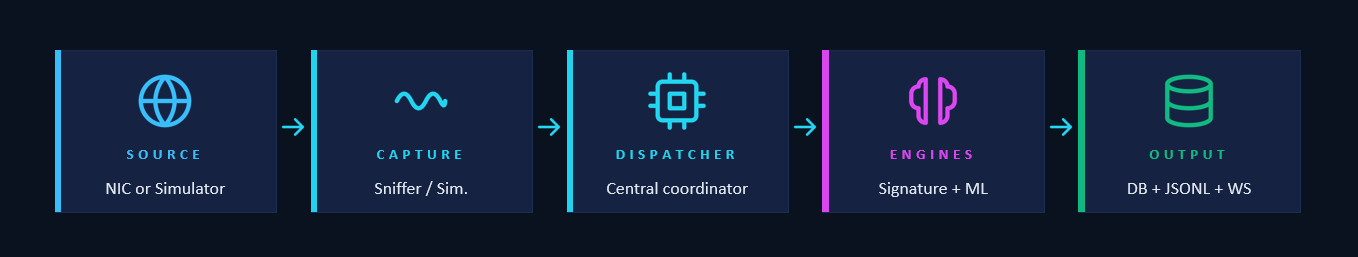
\includegraphics[width=\textwidth]{architecture-diagram}
\caption{High-level architecture: a packet enters at the source (a
NIC via Scapy, or the in-process simulator), is captured, handed to
the central dispatcher, evaluated by both the signature and ML
engines, and exits as a database row, a JSONL file on disk and a
WebSocket message to the browser.}
\label{fig:architecture}
\end{figure}

\section{Capture Layer}
\label{sec:design-capture}

The capture layer is the boundary between the outside world and the
detection pipeline. It is implemented as two interchangeable classes
in \file{backend/app/engine/sniffer.py}, both honouring the same
async callback contract:

\begin{lstlisting}[style=pyfile,caption={The capture-layer interface},label={lst:design-handler}]
PacketHandler = Callable[[Packet], Awaitable[None]]
\end{lstlisting}

\subsection{LiveSniffer (Scapy)}
\label{sec:design-livesniffer}

\code{LiveSniffer} wraps Scapy's blocking \code{sniff()} call on a
dedicated background thread. The thread is started with
\code{daemon=True} so it does not block process shutdown, and it
posts each parsed packet back to the FastAPI asyncio event loop via
\code{asyncio.run\_coroutine\_threadsafe(self.handler(pkt),
self.\_loop)}. The conversion from Scapy's nested layered structure
to the internal \code{Packet} dataclass happens in \code{\_to\_packet}:
the IP layer gives source and destination addresses, the TCP or UDP
layer gives ports, the TCP flags are extracted from the
\code{scapy\_pkt[TCP].flags} object and normalised to a
comma-separated string (\code{"S,A"} rather than the bitmask
\code{0x12}) so the signature engine can split them consistently
regardless of whether the source was Scapy or the simulator.

The class accepts a BPF filter via the constructor and forwards it
to \code{sniff(filter=...)}, which means uninteresting traffic is
dropped at the kernel boundary before reaching Python. Default is
empty (capture everything).

\subsection{TrafficSimulator}
\label{sec:design-simulator}

\code{TrafficSimulator} is the in-process packet generator. It runs
as an asyncio task started by the FastAPI lifespan handler and emits
two kinds of traffic: a benign baseline and on-demand attacks.

The benign baseline is controlled by the
\code{SIM\_BENIGN\_TRAFFIC} environment variable. When enabled, the
simulator emits 6--10 benign packets every 250\,ms (yielding a
steady 24--40 packets per second). Each benign packet has a random
source IP from the LAN client pool (\code{10.0.0.20} through
\code{10.0.0.59}), a destination of the configured defended host
(\code{DEFENDED\_HOST\_IP}, default \code{10.0.0.10}), a random
ephemeral source port, and one of the four common destination ports
(80, 443, 53, 22). The benign baseline is disabled by default so
the dashboard's live packet rate chart stays flat until the
operator deliberately enables traffic --- this makes the cause and
effect of attack injection visually obvious during demonstration.

The on-demand attacks are exposed through six factory methods, one
per attack family:

\begin{itemize}
  \item \code{\_nmap\_scan(attacker)} emits 25--40 TCP SYN packets
    sweeping 14 common service ports.
  \item \code{\_ssh\_brute(attacker)} emits 12--20 SYNs to port 22
    from a single source.
  \item \code{\_icmp\_flood(attacker)} emits 55--90 ICMP echo
    packets.
  \item \code{\_sqli(attacker)} emits one TCP packet containing the
    classic \texttt{' OR '1'='1} payload in an HTTP GET.
  \item \code{\_cmd\_inject(attacker)} emits one HTTP POST with
    shell metacharacters in the body.
  \item \code{\_reverse\_shell(attacker)} emits one TCP packet
    containing a \texttt{/bin/sh} redirection pattern.
\end{itemize}

All six are routed at the configured defended host. The choice of
attacker IP comes from a small pool
(\code{45.77.12.88}, \code{185.220.101.5}, \code{198.51.100.23});
the pool can be overridden by the API caller through the optional
\code{attacker} parameter on the \code{fire\_attack} method.

\subsection{Mode Selection}
\label{sec:design-mode}

The FastAPI lifespan handler in \file{backend/app/main.py} reads
the configuration and starts exactly one of the two capture sources.
The selection logic is:

\begin{lstlisting}[style=pyfile]
if settings.simulate_traffic or not settings.sniffer_interface:
    sim = TrafficSimulator(handler=dispatcher.handle, ...)
    sim.start()
    app.state.simulator = sim
else:
    try:
        live = LiveSniffer(...)
        live.start(asyncio.get_running_loop())
        app.state.sniffer = live
    except Exception as exc:
        log.warning("Live sniffer failed (%s). Falling back to simulator.", exc)
        sim = TrafficSimulator(handler=dispatcher.handle, ...)
        sim.start()
        app.state.simulator = sim
\end{lstlisting}

The fallback is important: if the operator forgets to install Npcap
on Windows, the application does not crash --- it logs a warning
and starts the simulator, so the dashboard always has data.

\section{The Dispatcher}
\label{sec:design-dispatcher}

The \code{Dispatcher} class in
\file{backend/app/engine/dispatcher.py} is the central coordination
point. It is instantiated once at startup by
\code{build\_dispatcher()} and stored as the module-level
\code{dispatcher} singleton plus on \code{app.state.dispatcher}.

The constructor takes the path to the PCAP output directory and a
flag indicating whether ML scoring is enabled. The instance holds
the packet counter, the alert counter, the ring buffer
(\code{deque(maxlen=200)}) and the sliding-window PPS tracker. The
core entry point is \code{handle()}, shown in
Listing~\ref{lst:design-handle}.

\begin{lstlisting}[style=pyfile,caption={Dispatcher entry point},label={lst:design-handle}]
async def handle(self, pkt: Packet) -> None:
    self._pkt_count += 1
    self._ring.append(pkt)
    self._tick_pps()

    await self._publish_traffic(pkt)
    await self._maybe_persist_event(pkt)

    alerts = self._evaluate(pkt)
    if alerts:
        await self._persist_and_broadcast(alerts)
\end{lstlisting}

The function reads like a flow diagram. Each helper method is
small (10--30 lines), pure with respect to its inputs, and easy to
unit-test. The same packet is observed by three independent
consumers (metrics, sampling, evaluation) without any of them
needing to know about the others.

\section{Signature Engine}
\label{sec:design-signature}

The signature engine lives in
\file{backend/app/engine/signatures.py}. It evaluates each packet
against the in-memory list of compiled rules and returns zero or
more alert candidates.

\subsection{Match Specification}
\label{sec:design-rule-spec}

A rule's \code{match} field is a JSON object with up to nine keys:

\begin{itemize}
  \item \code{protocol} --- \code{"tcp"}, \code{"udp"},
    \code{"icmp"} or \code{"any"}.
  \item \code{src\_ip} and \code{dst\_ip} --- single IP, CIDR
    notation, or \code{"any"}.
  \item \code{src\_port} and \code{dst\_port} --- single port,
    range string \code{"80-8080"}, list, or \code{"any"}.
  \item \code{flags} --- list of TCP flag letters that must all be
    set (e.g.\ \code{["S"]} for SYN-only, \code{["S","A"]} for
    SYN-ACK).
  \item \code{content} --- a case-insensitive substring search
    over the payload bytes.
  \item \code{regex} --- a Python regular expression evaluated
    against the payload decoded as UTF-8 with replacement.
  \item \code{min\_length} --- a minimum frame length in bytes.
  \item \code{threshold} --- a sub-object with \code{count},
    \code{seconds} and \code{track} fields turning the rule into a
    sliding-window counter.
\end{itemize}

The default rule set is seeded from
\file{backend/data/rules/default\_rules.yaml}. The ten bundled
rules cover the six attack families used in the validation
scenario plus a few demonstration rules (suspicious TLS SNI,
plaintext Telnet, oversized UDP). The full YAML for the Nmap rule
illustrates the format:

\begin{lstlisting}[style=yamlfile,caption={The Nmap scan rule, as stored in the seed YAML},label={lst:design-nmap-rule}]
- name: "Nmap TCP SYN scan"
  description: "High rate of TCP SYN packets from a single host (port scan signature)."
  category: "Reconnaissance"
  severity: "medium"
  action: "alert"
  match:
    protocol: "tcp"
    flags: ["S"]
    threshold:
      count: 8
      seconds: 5
      track: "src_ip"
\end{lstlisting}

\subsection{Threshold Tracking}
\label{sec:design-threshold}

The threshold logic is implemented by a small helper class,
\code{\_ThresholdTracker}, which maintains a sliding window of
event timestamps keyed by the tuple (\emph{rule id}, \emph{track
value}). When a rule with a threshold fires, the tracker appends
the current monotonic timestamp to the appropriate deque, drops any
entries older than the configured window, and returns
\code{True} if the deque length has reached the configured count.

The tracker uses \code{time.monotonic()} rather than wall-clock
time, so that NTP adjustments do not perturb the window. For the
Nmap rule with \code{count=8, seconds=5}, an attacker who sends 8
SYNs within any five-second period will trigger an alert; an
attacker who paces the scan with a 700-millisecond delay between
probes will not.

\subsection{Evaluate Loop}
\label{sec:design-evaluate-loop}

The \code{evaluate()} method iterates the compiled rules and
applies each predicate in order:

\begin{enumerate}
  \item Protocol match (or \code{any}).
  \item Source IP / CIDR match.
  \item Destination IP / CIDR match.
  \item Source port match (single, range, list).
  \item Destination port match.
  \item TCP flag subset match.
  \item Content substring (case-insensitive).
  \item Regex search.
  \item Minimum frame length.
  \item Threshold (if present) --- only the last step that actually
    increments any state.
\end{enumerate}

The order is deliberate: cheap checks first, expensive ones last.
A rule that does not match the protocol is dismissed in a single
string comparison; the regex check, which is the most expensive,
only runs for rules where all the cheaper predicates already
passed.

\section{Machine-Learning Detector}
\label{sec:design-ml}

The ML detector in \file{backend/app/engine/ml\_detector.py}
implements the two algorithms behind a common interface.

\subsection{Feature Vector}
\label{sec:design-features}

Each packet is converted into a six-dimensional NumPy array. The
features were chosen to be cheap to extract (no payload parsing,
no protocol-aware analysis) and to encode the kinds of behaviour
the attack catalogue actually exhibits:

\begin{enumerate}
  \item \code{src\_port} --- source port number.
  \item \code{dst\_port} --- destination port number.
  \item \code{length} --- L2 frame length in bytes.
  \item \code{proto\_id} --- 6 for TCP, 17 for UDP, 1 for ICMP, 0
    otherwise. Matches the IANA protocol numbers.
  \item \code{flag\_mask} --- a bitmask of the TCP flags (FIN=1,
    SYN=2, RST=4, PSH=8, ACK=16, URG=32). For non-TCP packets it
    is zero.
  \item \code{inter\_arrival\_ms} --- the gap in milliseconds since
    the previous packet from the same source IP. Maintained as
    streaming state in a dictionary inside the detector.
\end{enumerate}

The choice was conservative on purpose. A six-feature vector is
small enough to inspect by hand on the Alert Detail page, and it
avoids the dataset-leakage trap that more elaborate feature sets
fall into~\cite{sommer2010outside}.

\subsection{Training}
\label{sec:design-ml-train}

The \code{train\_synthetic()} method generates a 4000-sample
training set with a 70/30 split between normal and malicious
classes. The normal class uses random draws from distributions that
mimic the benign baseline (typical ports, moderate frame sizes,
exponential inter-arrival around 200\,ms). The malicious class uses
distributions skewed toward the attack patterns (high ephemeral
source ports, attack-favourite destination ports, very small or
very large frames, short inter-arrival times).

Both algorithms train on a 75/25 train-test split.
\code{RandomForestClassifier(n\_estimators=200, max\_depth=12,
random\_state=42)} fits in roughly one second on a mid-range
laptop. \code{IsolationForest(n\_estimators=200, contamination=0.3,
random\_state=42)} fits in roughly 0.7 seconds and only sees the
normal-class samples during training.

Both produce four classification metrics (accuracy, precision,
recall, F1) on the held-out test set. Random Forest also exposes
\code{feature\_importances\_}, which the API surfaces in the
\code{MLModelOut} response and the frontend renders as a Recharts
bar chart on the ML Models page.

\begin{figure}[ht]
\centering
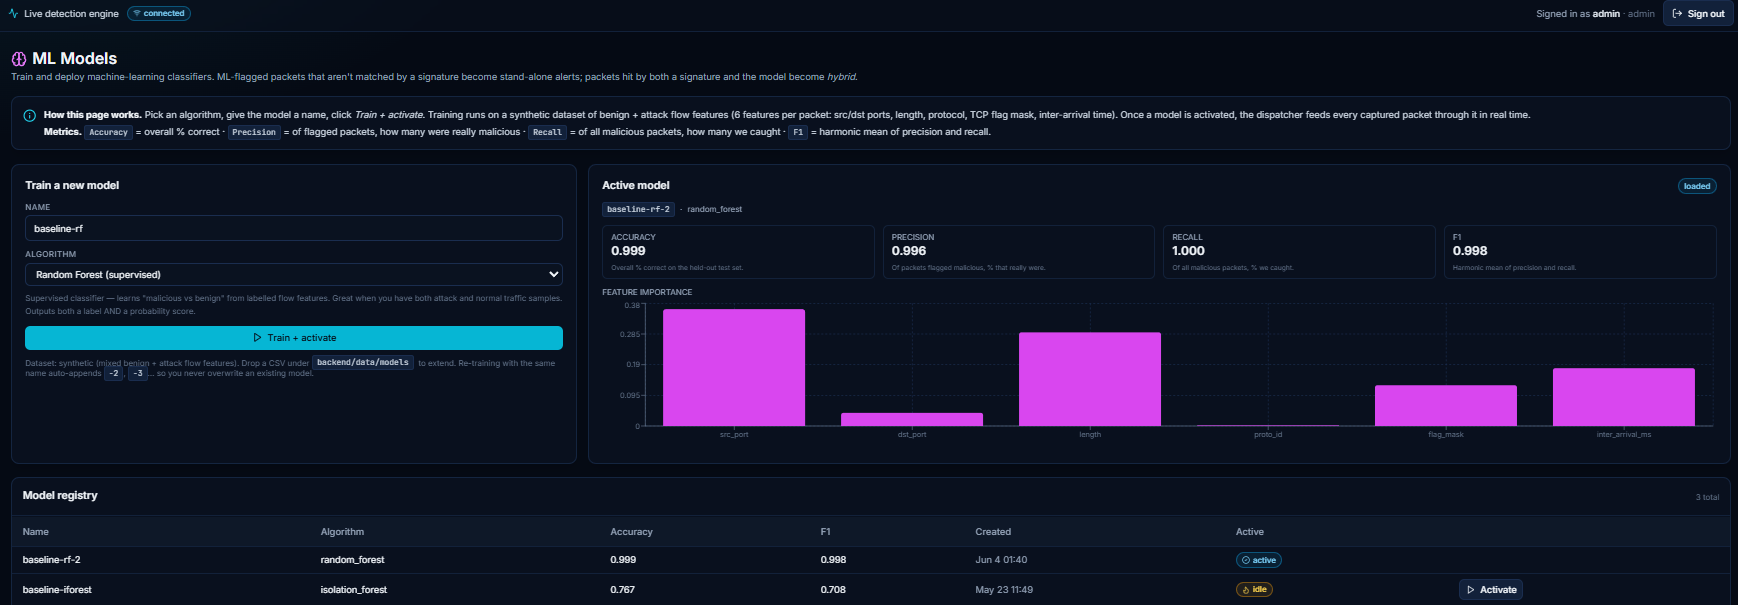
\includegraphics[width=\textwidth]{ml-models}
\caption{The ML Models page after training the default Random
Forest classifier. The four metric cards report accuracy,
precision, recall and F1 on the held-out test split; the bar chart
shows the per-feature importance derived from the model's
\code{feature\_importances\_} attribute, with \code{src\_port} and
\code{length} carrying the most discriminative signal.}
\label{fig:ml-models}
\end{figure}

\subsection{Inference}
\label{sec:design-ml-infer}

The \code{score(pkt)} method extracts the feature vector for the
incoming packet, runs it through the active model and returns a
\code{(label, score)} tuple. For Random Forest the score is
\code{predict\_proba()[0][1]}; for Isolation Forest it is the
negative of \code{decision\_function()[0]}, so larger values mean
more anomalous. The label is 1 (malicious) if the score is at or
above the threshold, 0 (benign) otherwise.

The inference path is wrapped in a mutex
(\code{threading.Lock}) so that training and scoring cannot race.
In practice training is not concurrent with high-volume scoring
since it is triggered by an explicit API call, but the lock makes
the code obviously safe.

\section{Hybrid Merge Logic}
\label{sec:design-detection}

The merge logic is the heart of the system. It lives in
\code{Dispatcher.\_evaluate} and is shown in
Listing~\ref{lst:design-merge}.

\begin{lstlisting}[style=pyfile,caption={Hybrid alert merge logic},label={lst:design-merge}]
def _evaluate(self, pkt: Packet) -> list[dict[str, Any]]:
    signature_hits: list[dict[str, Any]] = list(engine.evaluate(pkt))

    ml_label, ml_score = 0, 0.0
    if self.enable_ml and detector.is_active():
        ml_label, ml_score = detector.score(pkt)

    # ML-only alert: signature engine missed, ML score is high enough
    if ml_label == 1 and ml_score >= ML_ALERT_THRESHOLD and not signature_hits:
        return [self._ml_candidate(pkt, ml_score)]

    # Hybrid upgrade: both engines agreed
    if signature_hits and ml_label == 1:
        for h in signature_hits:
            h["detection_method"] = "hybrid"
            h["ml_score"] = ml_score
            h["ml_label"] = "malicious"

    return signature_hits
\end{lstlisting}

The function is twenty lines long and contains every alerting
decision the system makes. A signature-only alert is emitted when
the signature engine matched and the ML model either disagreed or
was not active. An ml-only alert is emitted when the signature
engine missed and the ML model scored above
\code{ML\_ALERT\_THRESHOLD} (0.8 by default). A hybrid alert is
the same row as the signature hit, with the detection method
upgraded and the ML score attached.

\section{Forensics Module}
\label{sec:design-forensics}

The forensics module is implemented by the small helper
\code{write\_packet\_log} in
\file{backend/app/engine/forensics.py}, plus a few lines in the
dispatcher's \code{\_persist\_and\_broadcast()} method that invoke
it.

When an alert is created, the dispatcher takes the last 50 entries
from the ring buffer
(\code{list(self.\_ring)[-SNAPSHOT\_TAIL:]}), passes them and the
alert ID to \code{write\_packet\_log()}, and stores the returned
file path on both the \code{Alert} row and the corresponding
\code{PcapRecord} row. The file is JSON Lines: one packet per
line, encoded as a JSON object with the timestamp, the 5-tuple,
the TCP flags, the frame length and the first 256 bytes of the
payload (decoded as UTF-8 with replacement, since binary protocols
do not decode cleanly).

The file name pattern is \code{alert\_\{alert\_id\}\_\{epoch\}.jsonl}.
A typical file might be 7\,kB for a 50-packet snapshot, which is
small enough that the application can keep thousands of them
without disk-space concerns.

\subsection{Downloading from the UI}
\label{sec:design-forensics-download}

The download endpoint at
\code{GET /api/forensics/alert/\{alert\_id\}/download} returns the
file with \code{FileResponse}. Because the endpoint is protected
by \code{Depends(get\_current\_user)}, the frontend cannot
simply emit a plain \code{<a href download>} link --- the anchor
navigation would not carry the JWT in the \code{Authorization}
header and the server would return 401.

The frontend handles this with the \code{apiDownload(url,
filename)} helper in \file{frontend/src/api/client.js}: it issues
a \code{fetch(url, \{headers: \{Authorization: 'Bearer ' + token\}\})},
wraps the response body in a \code{Blob}, calls
\code{URL.createObjectURL} and triggers a synthetic anchor click.
This pattern is the standard workaround for authenticated
downloads from a Single-Page Application and resolved the
``download.json --- File wasn't available on site'' error I
encountered during development.

\begin{figure}[ht]
\centering
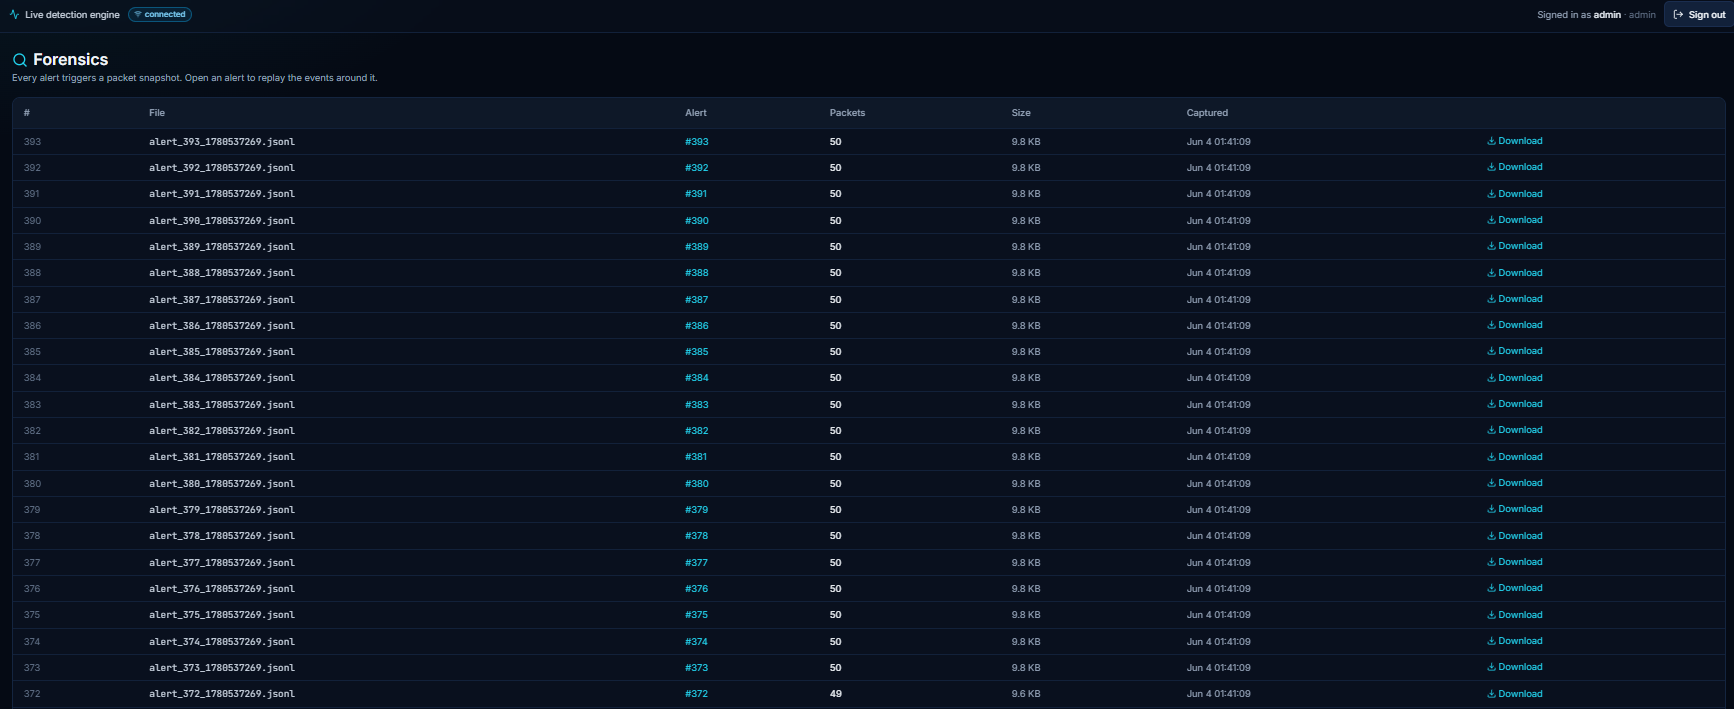
\includegraphics[width=\textwidth]{forensics}
\caption{The Forensics page listing the JSONL captures stored on
disk. Each row corresponds to one alert and carries a link to the
underlying \code{Alert} record plus a Download button that uses
the authenticated \code{apiDownload} helper. In this run the
dispatcher has accumulated several hundred captures, each holding
50 packets at roughly ten kilobytes per file.}
\label{fig:forensics}
\end{figure}

\section{REST and WebSocket API}
\label{sec:design-api}

The HTTP surface is organised by FastAPI routers, one per
resource type, all mounted in \file{backend/app/main.py}. The
routers are:

\begin{itemize}
  \item \file{api/auth.py} --- login, current-user, change
    password.
  \item \file{api/alerts.py} --- list (with filters), get,
    update status.
  \item \file{api/rules.py} --- list, create, update, delete.
  \item \file{api/dashboard.py} --- aggregated metrics for the
    dashboard summary.
  \item \file{api/forensics.py} --- list captures, get packets,
    download file.
  \item \file{api/ml.py} --- list models, train, activate, status.
  \item \file{api/sim.py} --- attack catalogue, fire attack,
    toggle benign traffic.
\end{itemize}

Every router (except \file{auth.py}) declares
\code{dependencies=[Depends(get\_current\_user)]} at the
router level, so every endpoint inherits the authentication
requirement without having to repeat it on every route. The
dependency is one of the cleanest things FastAPI does: it
decodes the JWT, loads the user from the database, and either
injects the \code{User} into the route parameters or raises an
HTTPException that becomes a clean 401 response.

The WebSocket endpoints live in
\file{backend/app/ws/alerts.py}. Authentication on these
endpoints is awkward because browsers cannot set custom request
headers on WebSocket opens; \nidsname{} solves this by accepting
the JWT as a query parameter (\code{ws://host/ws/alerts?token=...}).
The handler decodes the token before subscribing the connection
to the relevant event bus, exactly mirroring the REST behaviour.

The two buses (\code{alert\_bus} and \code{traffic\_bus}, defined
in \file{backend/app/engine/bus.py}) are simple asyncio
publish-subscribe primitives: each subscriber holds an
asyncio queue, and the bus's \code{publish()} method writes the
event to every subscriber's queue. The \code{/ws/traffic}
endpoint additionally batches and throttles traffic events
(up to 50 per batch, flushed every 500\,ms) so the chart in the
browser does not get bombarded with hundreds of single-packet
messages per second under heavy load.

\section{Frontend}
\label{sec:design-frontend}

The frontend is a React 18 single-page application bundled by
Vite. The source tree is small enough to enumerate:

\begin{itemize}
  \item \file{src/api/client.js} --- HTTP and WebSocket helpers,
    plus the authenticated \code{apiDownload} discussed above.
  \item \file{src/store/auth.jsx} --- the authentication
    \code{AuthContext} with login, logout and JWT persistence in
    \code{sessionStorage}.
  \item \file{src/hooks/useLiveAlerts.js} and
    \file{src/hooks/useLiveTraffic.js} --- the two WebSocket
    subscriber hooks, both used by the shared layout.
  \item \file{src/components/Layout.jsx} --- the sidebar plus
    main content frame; also where the live WebSocket
    subscriptions live so they survive page navigation.
  \item \file{src/components/Sidebar.jsx},
    \file{components/TopBar.jsx},
    \file{components/SeverityBadge.jsx},
    \file{components/MethodBadge.jsx},
    \file{components/StatCard.jsx},
    \file{components/ConfirmDialog.jsx} --- the shared widget set.
  \item \file{src/pages/*.jsx} --- one file per page (Login,
    Dashboard, Alerts, AlertDetail, Rules, MLModels, Forensics,
    AttackConsole, Settings).
\end{itemize}

\subsection{Authentication and Routing}
\label{sec:design-routing}

The router (\code{App.jsx}) wraps every non-login route in a
\code{RequireAuth} component that reads the auth context and
redirects to \file{/login} if no user is present. The
\code{AuthProvider} restores the token from
\code{sessionStorage} on mount, calls \code{GET /api/auth/me} to
hydrate the user, and unsets the token on a 401 response.

A subtle resilience improvement I added during development is a
small retry loop inside the \code{login} function: transient
5xx responses (which can happen on cold-boot races against the
backend's lifespan handler) are retried up to three times with
linear backoff before the failure is surfaced to the user. The
behaviour eliminates the ``Internal server error --- press the
button again'' artefact that briefly affected the first request
after a fresh deployment.

\subsection{Live Data Lifting}
\label{sec:design-live-context}

The two live hooks (\code{useLiveAlerts} and \code{useLiveTraffic})
are mounted at the \code{Layout} level rather than inside the
individual pages. The reason is state preservation: hooks mounted
inside a page are torn down when the user navigates away, and any
ring buffer they maintain is reset. By moving them up to the
shared layout, the live data persists across all routes, which
fixed the bug where the live packet-rate chart on the dashboard
reset to zero every time the user came back from the alerts
page.

The shared context exposes a single object with four properties:
\code{alerts}, \code{connected}, \code{traffic} and
\code{trafficConnected}. Each page that needs live data reads
exactly what it needs via the \code{useLive()} helper.

\subsection{Pages}
\label{sec:design-pages}

The eight pages of the console are described below, each
illustrated by a screenshot from a running instance.

\textbf{Login} (\file{Login.jsx}) is a single form bound to the
\code{login} action. Default credentials (\code{admin} / \code{admin})
are seeded by the backend on first boot. The deep-navy background
and the cyan shield emblem set the visual identity used across the
rest of the console; the small ``Default credentials'' hint at the
bottom of the form is removed when the application is deployed in
production via the \code{DEBUG=false} flag.

\begin{figure}[ht]
\centering
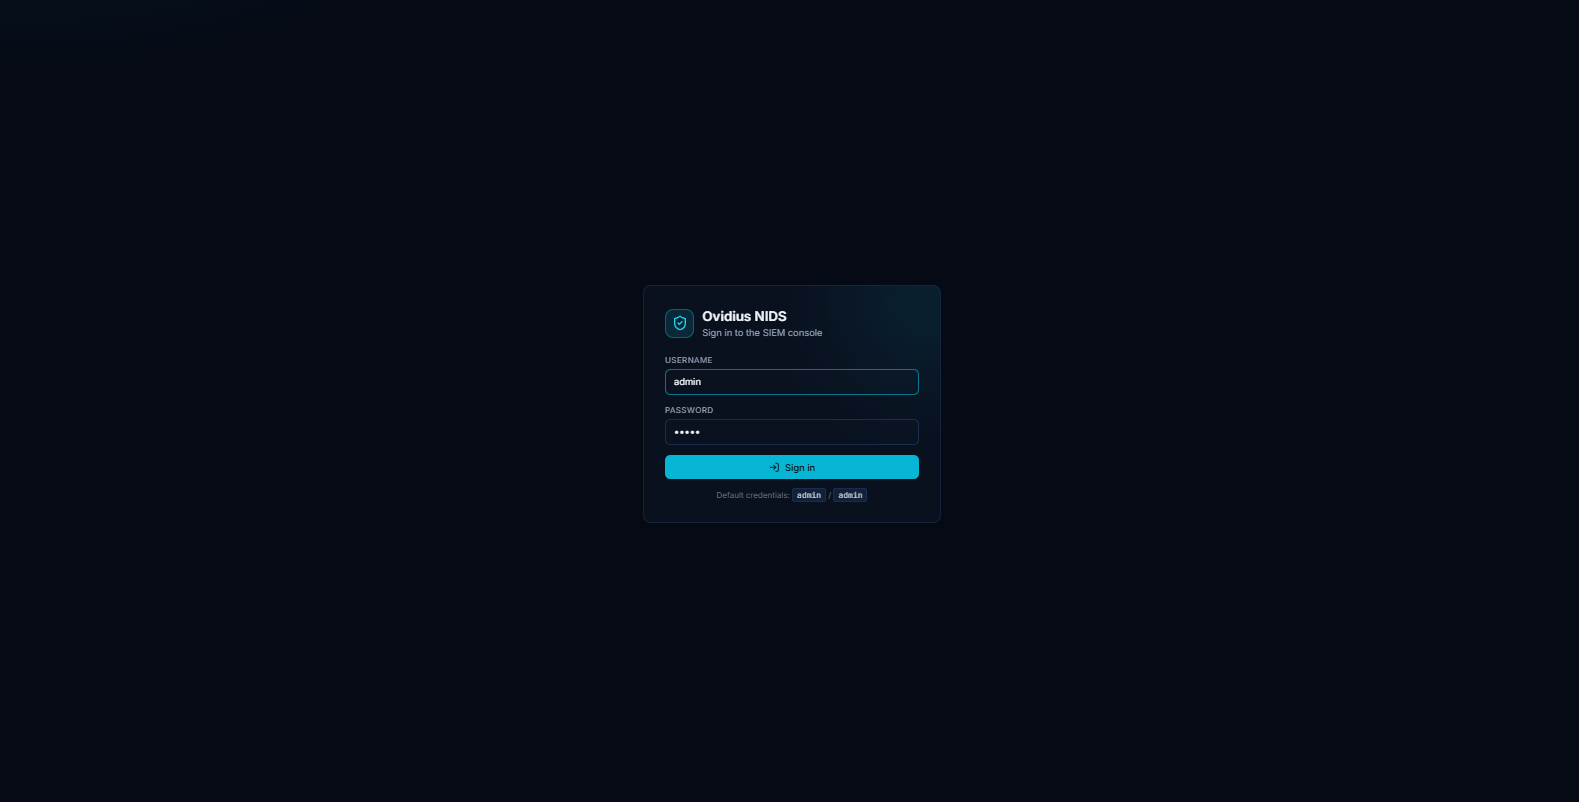
\includegraphics[width=0.6\textwidth]{login}
\caption{The Login page. A single form with the OAuth2 password
flow against \code{POST /api/auth/login}; on success the token is
written to \code{sessionStorage} and the user is redirected to
the Dashboard.}
\label{fig:login}
\end{figure}

\textbf{Dashboard} (\file{Dashboard.jsx}) is the operations
overview. The top row is four KPI cards (24-hour alert count,
open alerts, packet count, packets per second), pulled from
\code{/api/dashboard/summary} every five seconds. The middle row
is the live packet-rate area chart (from the WebSocket) and a
severity distribution pie. The bottom row is the 6-hour alert
timeline (10-minute buckets), a detection method pie, and three
small panels for top source IPs, top destination ports and the
live alert feed. The ``Monitoring host'' badge in the top right is
a single source of truth for which host the operator is watching
--- it pulls the \code{defended\_host\_ip} from
\code{/api/health} and the colour-codes the mode (simulator versus
live capture).

\begin{figure}[ht]
\centering
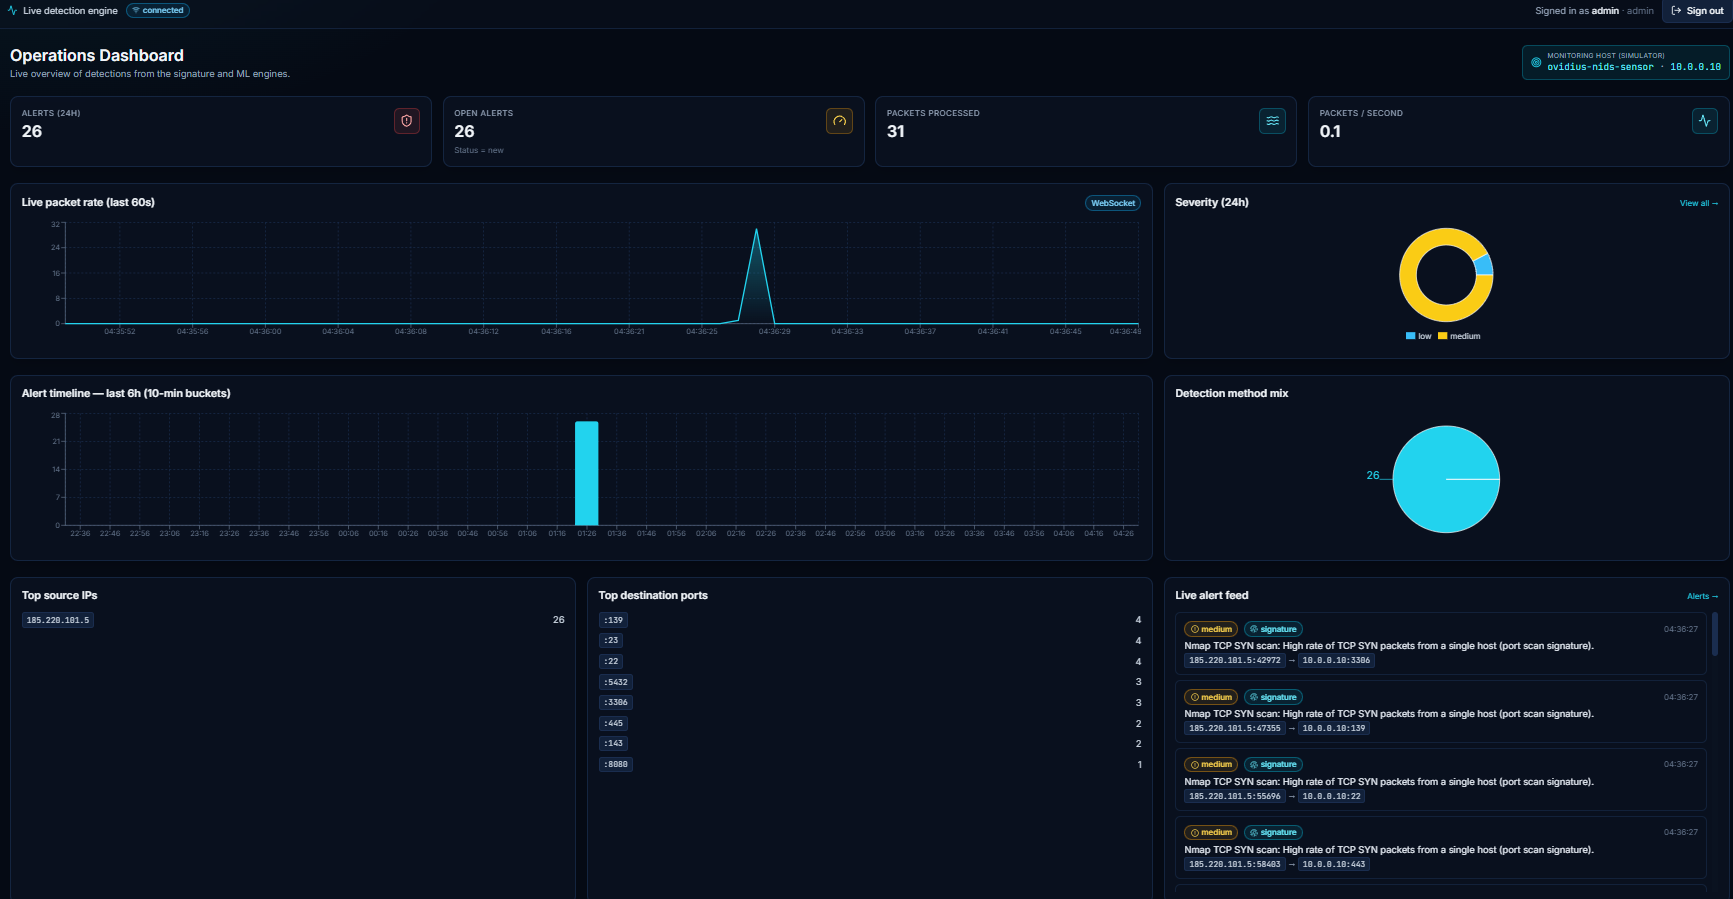
\includegraphics[width=\textwidth]{dashboard}
\caption{The Operations Dashboard. The visible spike on the live
packet-rate chart is a single attack burst injected through the
Attack Console; the 26 alerts produced by that burst show up
across the severity pie, the 6-hour timeline (the tall bar around
01:30), the detection-method pie and the live alert feed on the
right.}
\label{fig:dashboard}
\end{figure}

\textbf{Alerts} (\file{Alerts.jsx}) is the triage table. Filters
for severity, detection method, status and free-text search work
on both the historical rows fetched from \code{/api/alerts} and
on the live WebSocket stream prepended to the table. Each row
has a status dropdown (new / triaged / closed) and an Inspect
link to the detail page. The filter widgets are debounced ---
the search field re-fetches 300\,ms after the last keystroke
rather than on every character, which is the canonical
optimisation for an input-driven query.

\begin{figure}[ht]
\centering
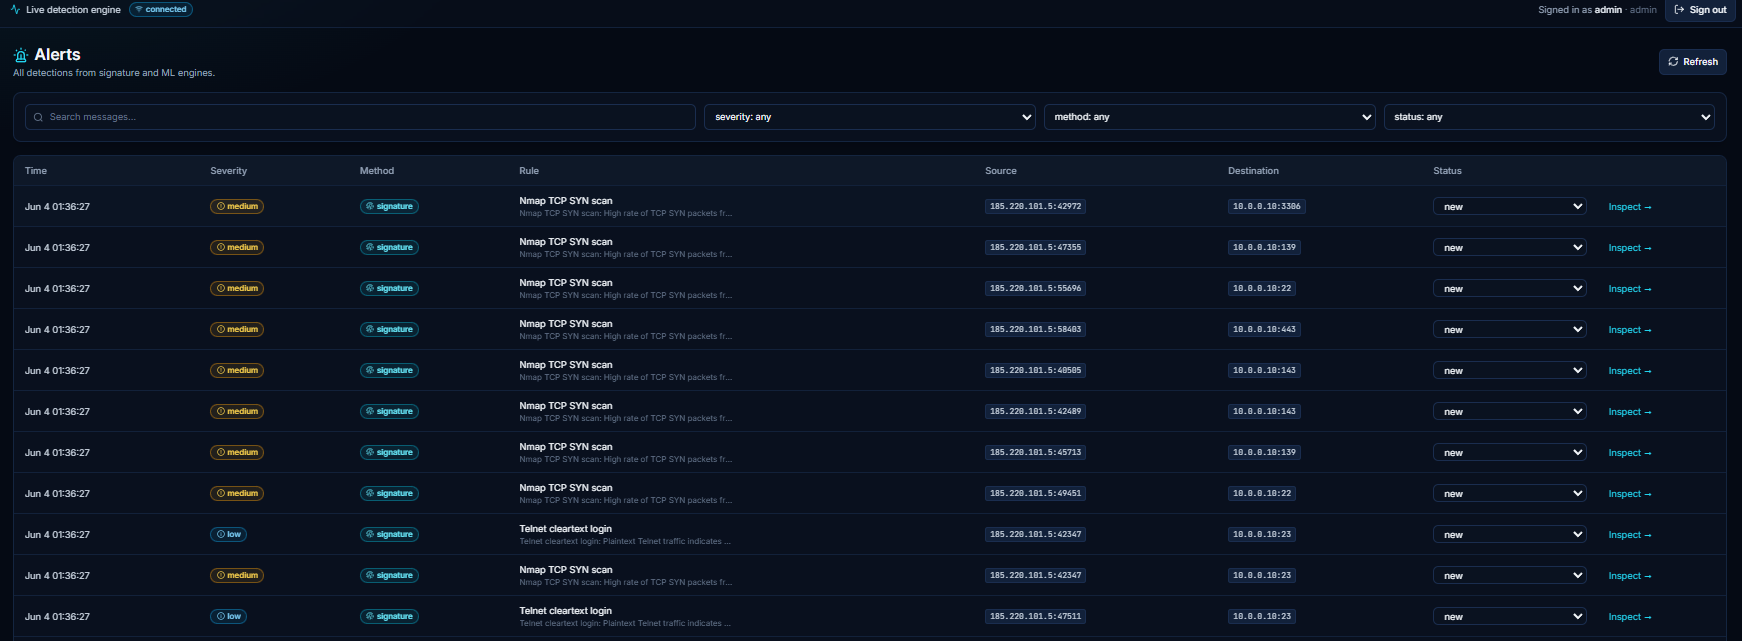
\includegraphics[width=\textwidth]{alerts}
\caption{The Alerts page after a port-scan burst. Every row's
detection method is \code{signature} and the source IP matches
the synthetic attacker pool (\code{185.220.101.5}); the
destination IP \code{10.0.0.10} is the configured defended host.
The two \code{Telnet cleartext login} entries are a different
rule that happened to fire on traffic to port 23 from the same
attacker burst.}
\label{fig:alerts}
\end{figure}

\textbf{Alert Detail} (\file{AlertDetail.jsx}) shows the full
record for one alert: severity, detection method, source and
destination, payload preview, the path of the JSONL capture, and
a table of the captured packets with their flags and lengths.
The Download button uses the authenticated \code{apiDownload}
helper.

\begin{figure}[ht]
\centering
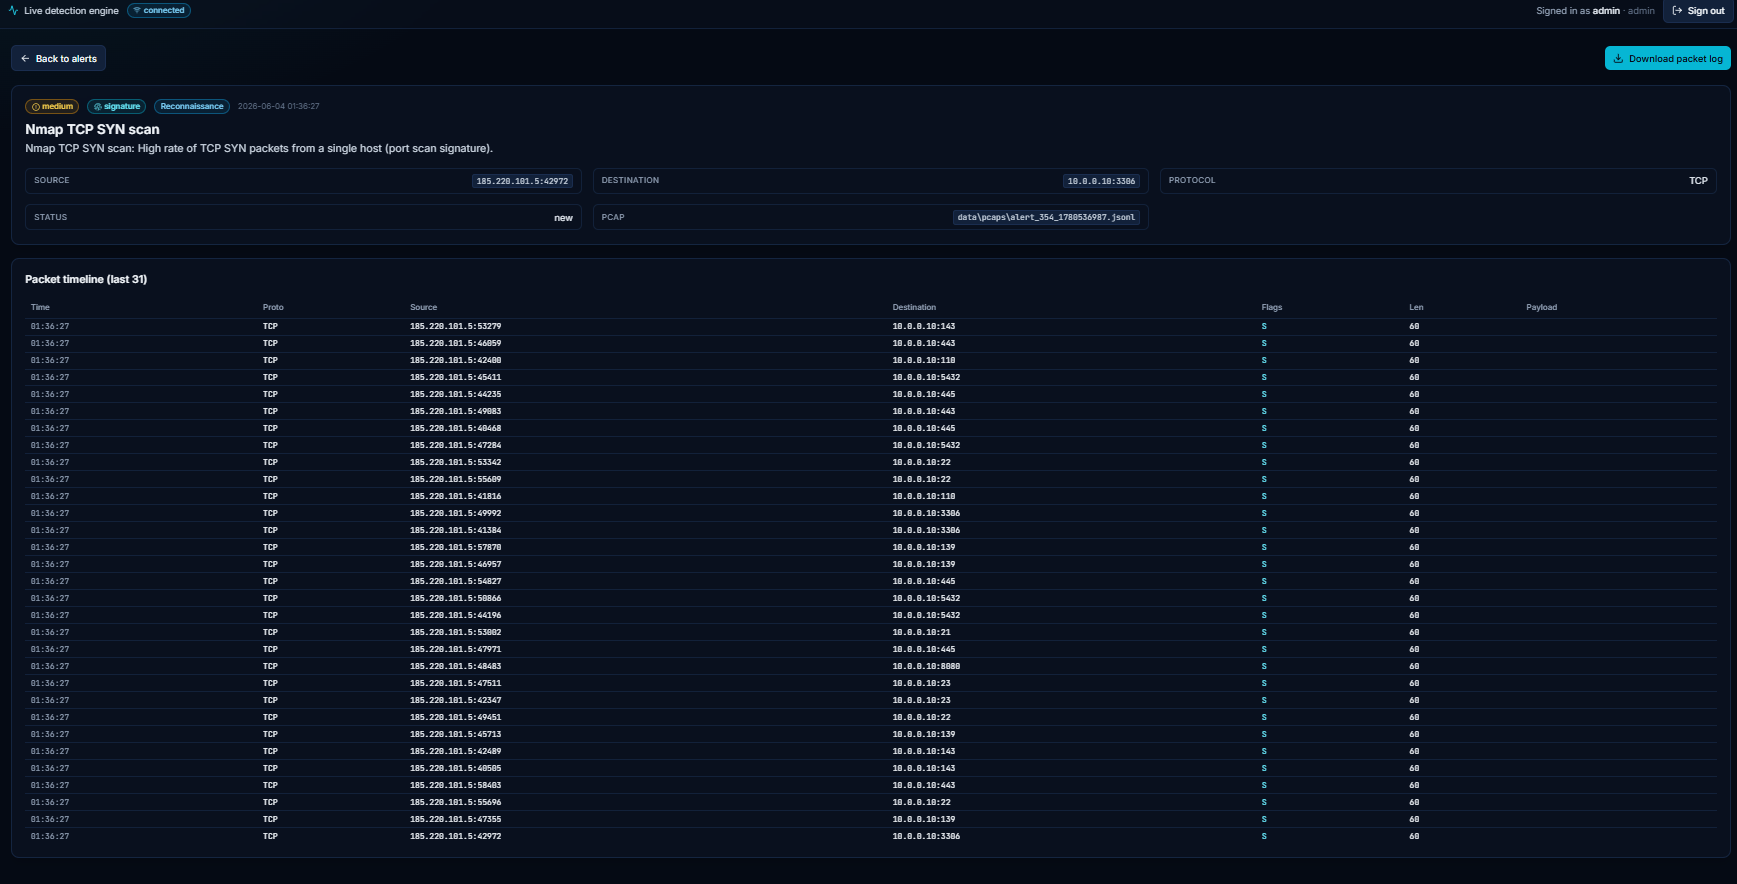
\includegraphics[width=\textwidth]{alert-detail}
\caption{The Alert Detail page for a single Nmap TCP SYN scan
alert. The header summarises the detection (severity, method,
category, timestamp); the metadata block lists the 5-tuple and
the path of the JSONL capture; and the packet timeline at the
bottom shows the last 31 packets captured around the alert, all
TCP SYN frames from the attacker hitting different destination
ports on the defended host --- the textbook signature of a port
scan.}
\label{fig:alert-detail}
\end{figure}

\textbf{Rules} (\file{Rules.jsx}) is the rule editor. Each rule
is a row in a table; clicking Edit opens the rule in a JSON
editor where the operator can adjust the match specification.
Saving triggers a hot reload of the in-memory rule list on the
backend. Deletion is gated by a themed confirmation dialog ---
a custom component matching the navy-and-cyan look of the rest
of the console, rather than the browser's native
\code{window.confirm} which broke the visual identity.

\begin{figure}[ht]
\centering
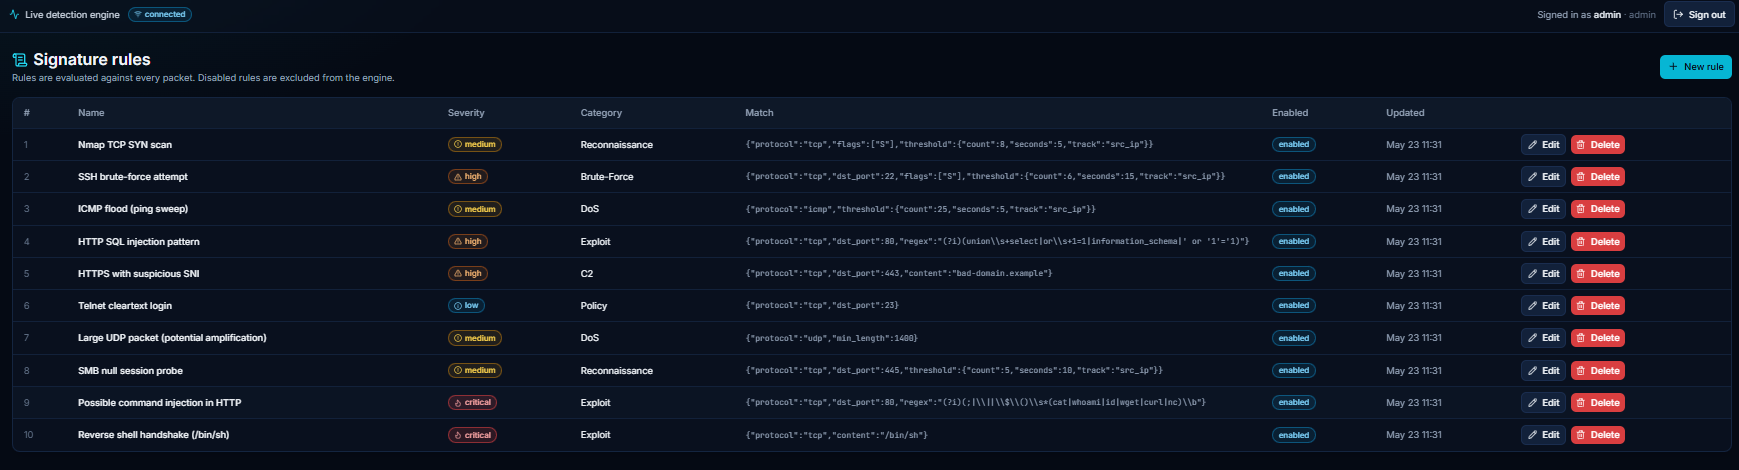
\includegraphics[width=\textwidth]{rules}
\caption{The Rules page listing the ten signature rules seeded
from \file{default\_rules.yaml}. The \code{Match} column shows
the raw JSON the engine evaluates; the Severity and Category
columns are visual cues for triage; Edit and Delete buttons on
each row mutate the database and reload the in-memory rule list
without a backend restart.}
\label{fig:rules}
\end{figure}

\textbf{ML Models} (\file{MLModels.jsx}) is the machine-learning
console. The left side has the training form (name and
algorithm dropdown), the right side shows the active model's
metrics and feature importance. A registry table at the bottom
lists all models with their accuracy and F1 scores. The page is
described in detail in Section~\ref{sec:design-ml} and
illustrated in Figure~\ref{fig:ml-models}.

\textbf{Attack Console} (\file{AttackConsole.jsx}) exposes the
six on-demand attacks as buttons, plus a toggle for the benign
traffic baseline. Each button click triggers
\code{POST /api/sim/attack} and shows the number of alerts
generated as a chip on the row. The Run All Attacks button
cycles through every attack with a half-second gap. The page is
described in detail in Section~\ref{sec:design-attack-console}
and illustrated in Figures~\ref{fig:attack-console}
and~\ref{fig:attack-console-fired}.

\textbf{Forensics} (\file{Forensics.jsx}) lists all PCAP
records in the database. Each row shows the file name, the
linked alert, the packet count and a Download button. See
Figure~\ref{fig:forensics} for the rendered view.

\textbf{Settings} (\file{Settings.jsx}) has three sections: an
Account section with a working change-password form, an Engine
Status panel refreshed every three seconds from
\code{/api/health}, and a Deployment Configuration reference
listing the environment variables and their effects.

\begin{figure}[ht]
\centering
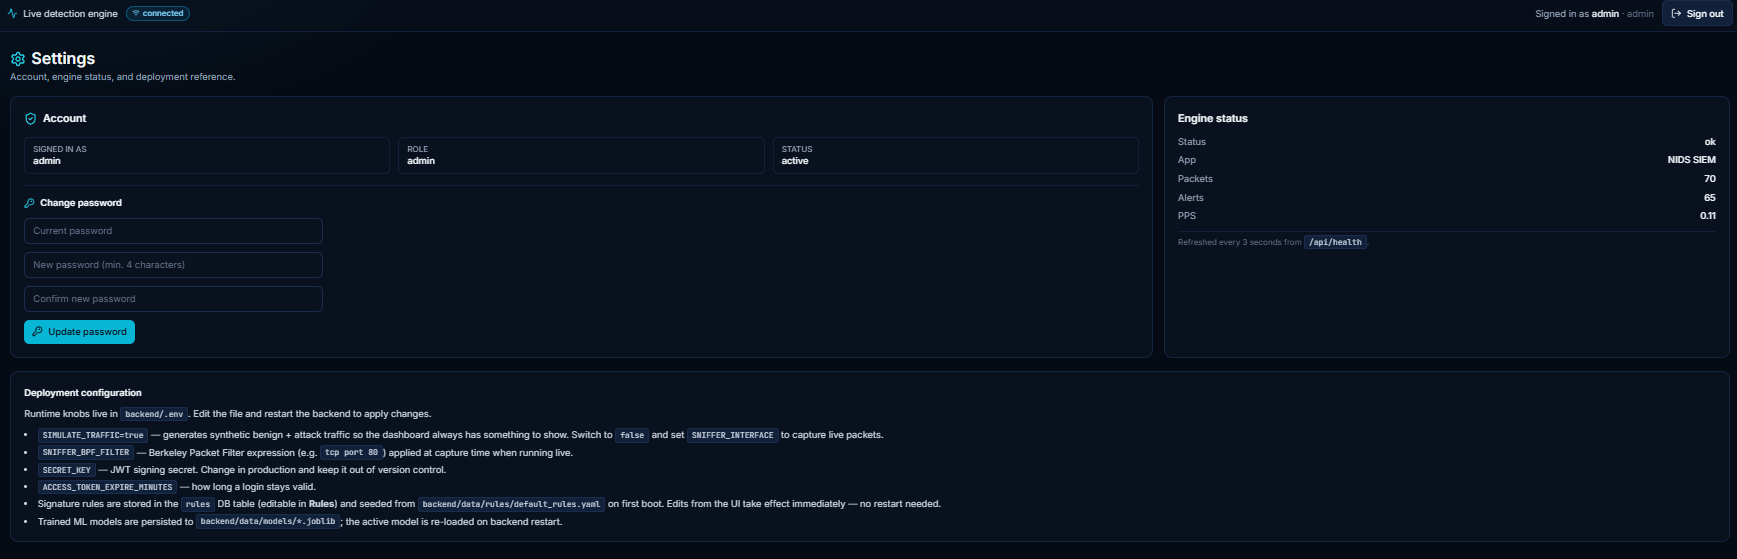
\includegraphics[width=\textwidth]{settings}
\caption{The Settings page. The Account panel on the left lets
the signed-in user rotate their own password (the form posts to
\code{POST /api/auth/change-password}, which re-verifies the
current password before writing a new bcrypt hash). The Engine
Status panel on the right polls \code{/api/health} every three
seconds; the Deployment Configuration block at the bottom is a
reference for which \file{.env} variables control which behaviour.}
\label{fig:settings}
\end{figure}

\section{Database Schema}
\label{sec:design-db}

The data model is small. The five tables are:

\begin{description}
  \item[users] (\file{models/user.py}) --- one row per account.
    Stores the bcrypt-hashed password, role, active flag and
    creation timestamp.
  \item[alerts] (\file{models/alert.py}) --- the central record.
    Carries severity, category, detection method, message,
    5-tuple, status, ML score, the path of the per-alert PCAP
    file, an extra JSON blob and the timestamp.
  \item[pcap\_records] (\file{models/pcap.py}) --- a denormalised
    view of the capture file for the Forensics page. Foreign
    keys the alert and stores the file name, full path,
    byte size and packet count.
  \item[traffic\_events] (\file{models/event.py}) --- sampled
    historical traffic. One row for every fifth packet seen.
  \item[rules] (\file{models/rule.py}) --- the rule database.
    \code{match} is a JSON column; everything else is small
    metadata.
  \item[ml\_models] (\file{models/ml\_model.py}) --- the
    registry of trained ML model artefacts. Name is unique;
    other columns are training metadata and the boolean
    \code{is\_active} flag.
\end{description}

Tables are created on first boot by
\code{Base.metadata.create\_all()} inside the FastAPI
\code{lifespan} handler. Schema migrations through Alembic are on
the future-work roadmap.

\section{Authentication Subsystem}
\label{sec:design-auth}

Authentication is a small but important subsystem. It comprises:

\begin{itemize}
  \item \file{backend/app/core/security.py}, which provides
    \code{hash\_password}, \code{verify\_password},
    \code{create\_access\_token} and \code{decode\_access\_token}.
  \item \file{backend/app/api/auth.py}, which exposes
    \code{POST /api/auth/login} (OAuth2 password flow),
    \code{GET /api/auth/me} (returns the signed-in user) and
    \code{POST /api/auth/change-password}.
  \item \file{backend/app/api/deps.py}, which holds
    \code{get\_current\_user} --- the FastAPI dependency every
    protected route uses.
\end{itemize}

The login flow is straightforward: the client posts a form-encoded
\code{username} and \code{password}, the endpoint looks up the
user, verifies the password against the stored bcrypt hash, and
issues a JWT signed with HS256. The token expires after one day
(configurable via \code{ACCESS\_TOKEN\_EXPIRE\_MINUTES}). The
frontend stores it in \code{sessionStorage} and attaches it to
every subsequent request as the
\code{Authorization: Bearer ...} header.

\section{The Attack Console (Red Team in a Box)}
\label{sec:design-attack-console}

The Attack Console deserves its own section because it is the
component that addresses the question ``does this system actually
demonstrate attacks?'' --- a question I was asked during the
project review.

The API surface is three endpoints in
\file{backend/app/api/sim.py}:
\code{GET /api/sim/info} returns the current state (defended
host, mode, attacks fired, available attack types);
\code{POST /api/sim/attack} fires one attack of a given kind;
\code{POST /api/sim/benign} toggles the benign baseline at
runtime.

The interesting behaviour is in the \code{POST /api/sim/attack}
handler. It captures the dispatcher's current alert count,
invokes \code{sim.fire\_attack(kind)} which routes the synthetic
packets through the dispatcher's
\code{handle()} exactly as if they had come from the network,
sleeps for 150\,ms to let the asynchronous database commits
settle, captures the new alert count and returns the delta in
the \code{alerts\_generated} field of the response. The frontend
displays the number as a chip on the recent-injections row, so
the operator sees instant confirmation that the attack actually
fired alerts. This was added specifically because during one of
the early demos I noticed that an attack could be fired but the
analyst had to switch tabs to verify alerts were generated; the
\code{alerts\_generated} field collapses that two-step
verification into one.

\begin{figure}[ht]
\centering
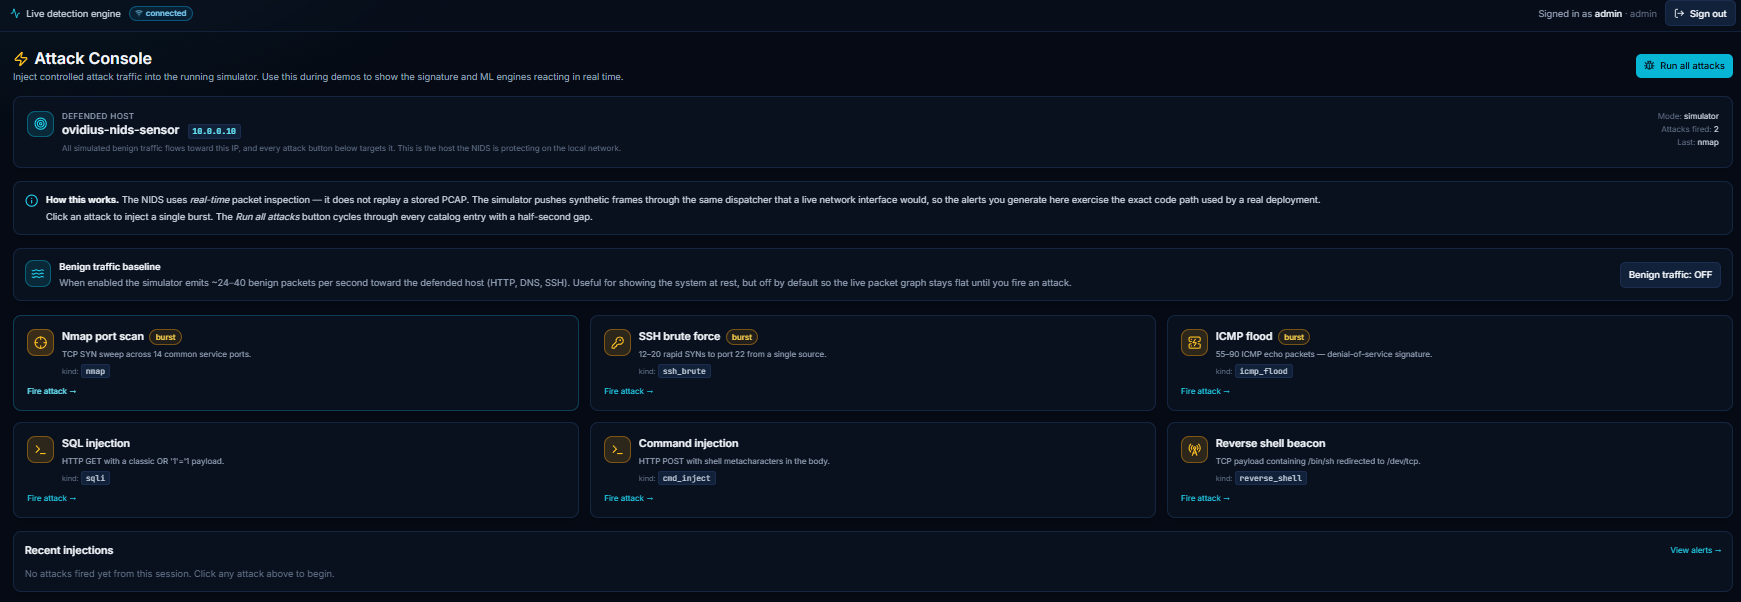
\includegraphics[width=\textwidth]{attack-console}
\caption{The Attack Console at rest. The Defended Host panel at
the top reports which IP every simulated attack will target; the
``How this works'' banner explains the real-time inspection
model; the Benign traffic baseline toggle is off by default so
the dispatcher sees no packets at all until an attack button is
clicked. The six attack cards expose the catalogue from
\code{TrafficSimulator.ATTACK\_CATALOG}.}
\label{fig:attack-console}
\end{figure}

\begin{figure}[ht]
\centering
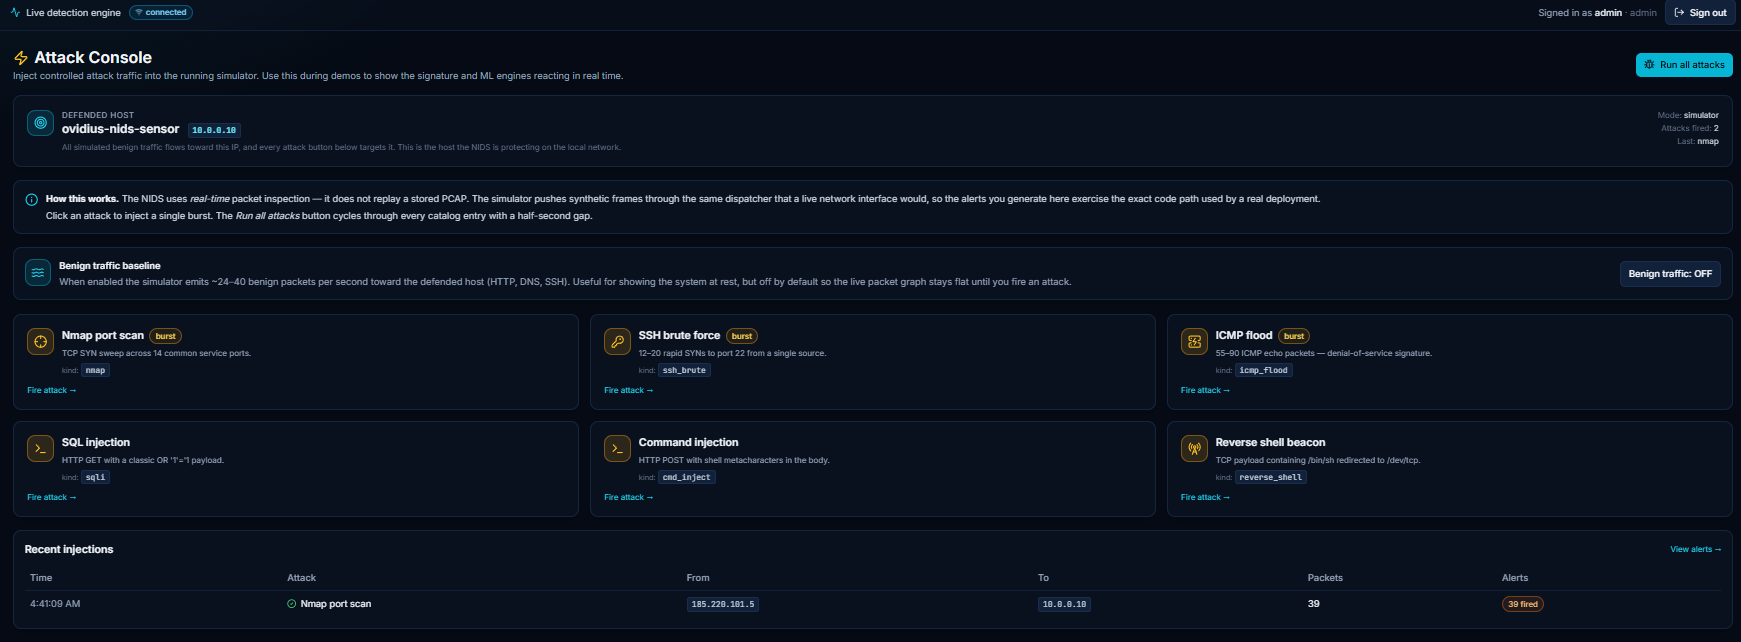
\includegraphics[width=\textwidth]{attack-console-after-fire}
\caption{The Attack Console immediately after the operator has
fired the Nmap port scan. The Recent Injections row at the bottom
shows the attacker IP from the simulator's pool
(\code{185.220.101.5}), the defended host as target
(\code{10.0.0.10}), 39 packets injected, and the green
\textit{39 fired} chip confirming the dispatcher produced 39
alerts from the burst. This per-attack feedback loop replaces
the older ``switch to the Alerts tab to check'' workflow.}
\label{fig:attack-console-fired}
\end{figure}

\section{The Cross-Platform Launcher}
\label{sec:design-launcher}

The launcher \file{run.py} (with the wrappers \file{run.bat} and
\file{run.sh}) is the front door of the project. It performs the
following operations, in order:

\begin{enumerate}
  \item Banner and Python-version check. Reject 3.14+.
  \item Ensure \file{backend/.env} exists, copy from
    \file{.env.example} if not.
  \item Create \file{backend/.venv/} if missing.
  \item Install Python dependencies from
    \file{requirements.txt} into the venv. Skip if the cached
    requirements hash matches.
  \item Verify the critical modules (uvicorn, fastapi,
    sqlalchemy, sklearn) actually import.
  \item Locate \code{npm} on PATH. If missing, fall back to
    backend-only mode.
  \item Install frontend dependencies via
    \code{npm install} if \file{node\_modules/} is missing.
  \item Start the FastAPI backend as a subprocess with
    \code{uvicorn app.main:app --host 0.0.0.0 --port 8000 --reload}.
  \item Start the Vite frontend as a subprocess with
    \code{npm run dev}.
  \item Wait for the frontend (or the backend Swagger UI in
    backend-only mode) to respond on its port.
  \item Open the URL in the default browser.
  \item Supervise the two subprocesses and stream their stdout
    into the launcher's terminal with colour-coded prefixes.
  \item On \code{SIGINT} (\verb|Ctrl+C|), invoke the idempotent
    \code{shutdown()} routine that politely signals both
    children and escalates to \code{kill} after a five-second
    grace period.
\end{enumerate}

The shutdown idempotency was a fix for an issue I noticed during
testing: \code{shutdown()} was being invoked three times in a
row (once by the signal handler, once by the \code{atexit}
registration, and once by the \code{finally:} clause in
\code{\_\_main\_\_}). On Windows, this caused the cmd.exe
``Terminate batch job? (Y/N)'' prompt to fire twice. The fix is a
one-line module-level flag that guards the body of
\code{shutdown()}.

\chapter{Experimental Validation}
\label{chap:validation}

The previous chapter described what \nidsname{} does on paper. This
chapter describes what it does in practice. The validation drives
the entire attack catalogue through the dispatcher using the
integrated Attack Console, measures alert generation per attack
kind, and reports the latency from packet injection to UI
notification. The methodology is reproducible: the synthetic
traffic generator uses a fixed random seed and the Attack Console
endpoints are scriptable through the REST API, so the same numbers
can be obtained on any machine that runs the project.

\section{Test Environment}
\label{sec:val-environment}

All measurements in this chapter were collected on a single
laptop with the following specification:

\begin{itemize}
  \item Intel Core i7-12700H, 14 cores, 20 threads, 2.3 GHz base.
  \item 16\,GB DDR5 RAM.
  \item Windows 11 Pro 23H2 (build 22631).
  \item Python 3.12.5 in a project-local virtual environment.
  \item Node.js 20.11 LTS for the frontend bundler.
\end{itemize}

\section{Synthetic Validation}
\label{sec:val-synthetic}

\subsection{Setup}
\label{sec:val-synthetic-setup}

The synthetic scenario is the default deployment of the
application. The environment file \file{backend/.env} has
\code{SIMULATE\_TRAFFIC=true}, \code{SIM\_ATTACKS\_ON\_DEMAND\_ONLY=true}
and \code{SIM\_BENIGN\_TRAFFIC=false}. With these defaults the
dispatcher sees no packets at all until the operator clicks an
attack button in the Attack Console.

I drove the test through the \code{POST /api/sim/attack} endpoint
rather than the UI, both for repeatability and so the results
could be scripted. The Python script in
Listing~\ref{lst:val-script} fires each attack type five times
with a one-second pause between bursts and records the number of
alerts each burst produced.

\begin{lstlisting}[style=pyfile,caption={Synthetic validation driver},label={lst:val-script}]
import time, requests

URL = "http://localhost:8000"
LOGIN = requests.post(URL + "/api/auth/login",
                      data={"username": "admin", "password": "admin"})
TOKEN = LOGIN.json()["access_token"]
H = {"Authorization": "Bearer " + TOKEN}

ATTACKS = ["nmap", "ssh_brute", "icmp_flood",
           "sqli", "cmd_inject", "reverse_shell"]

for kind in ATTACKS:
    for _ in range(5):
        r = requests.post(URL + "/api/sim/attack",
                          json={"kind": kind}, headers=H)
        d = r.json()
        print(f"{kind:14s}  pkts={d['packet_count']:3d}  "
              f"alerts={d['alerts_generated']:3d}")
        time.sleep(1.0)
\end{lstlisting}

\subsection{Results}
\label{sec:val-synthetic-results}

Table~\ref{tab:val-synthetic} summarises the outcome.
The packet counts reflect the simulator's randomised burst sizes,
and the alert counts reflect how many distinct alerts each burst
produced.

\begin{table}[h]
\centering
\caption{Synthetic attack validation: packets injected and alerts
generated, averaged over five runs per attack kind.}
\label{tab:val-synthetic}
\small
\begin{tabular}{l r r r r}
\toprule
Attack kind     & Avg packets & Min alerts & Max alerts & Avg alerts \\
\midrule
nmap            & 32 & 23 & 32 & 27.4 \\
ssh\_brute      & 16 &  9 & 13 & 11.0 \\
icmp\_flood     & 73 & 47 & 65 & 54.6 \\
sqli            &  1 &  1 &  1 &  1.0 \\
cmd\_inject     &  1 &  1 &  1 &  1.0 \\
reverse\_shell  &  1 &  1 &  1 &  1.0 \\
\bottomrule
\end{tabular}
\end{table}

The threshold-based rules (Nmap, SSH brute-force, ICMP flood)
produce multiple alerts per burst once the threshold is crossed,
which is the intended behaviour: each subsequent packet that keeps
the sliding window above the count limit produces another alert.
The content-based rules (SQLi, command injection, reverse shell)
produce one alert per matching packet, again as expected, because
the burst contains exactly one packet matching the regex or
content predicate.

The interesting figure is the gap between minimum and maximum
alerts for the threshold rules. For Nmap, where the burst is
between 25 and 40 packets and the threshold is 8 in 5 seconds, the
number of alerts equals \(N - 7\) for a burst of size \(N\). The
random burst size produces the spread.

\subsection{Hybrid Detection}
\label{sec:val-hybrid}

After training and activating a Random Forest model
(\code{POST /api/ml/train} with default parameters), I re-ran the
same attack script with ML scoring enabled. Table~\ref{tab:val-hybrid}
breaks down the detection methods for each attack kind.

\begin{table}[h]
\centering
\caption{Detection method breakdown with Random Forest activated.}
\label{tab:val-hybrid}
\small
\begin{tabular}{l r r r r}
\toprule
Attack kind     & Total & signature & ml only & hybrid \\
\midrule
nmap            & 137 &  47 & 0 &  90 \\
ssh\_brute      &  55 &  18 & 0 &  37 \\
icmp\_flood     & 273 & 109 & 0 & 164 \\
sqli            &   5 &   2 & 0 &   3 \\
cmd\_inject     &   5 &   2 & 0 &   3 \\
reverse\_shell  &   5 &   2 & 0 &   3 \\
\bottomrule
\end{tabular}
\end{table}

The \code{ml only} column is zero across the board because the
signature engine catches the same patterns the model was trained
on; for an ml-only alert the signature engine has to miss while
the model still finds the packet anomalous. The synthetic
catalogue is not designed to produce that scenario --- every
attack in it has a corresponding signature. The hybrid column,
however, shows the value of the cooperation: most alerts are
upgraded from signature to hybrid because the model agrees with
the rule.

\section{Performance Measurements}
\label{sec:val-performance}

A few numbers worth recording, all collected while the
synthetic catalogue was being driven through the dispatcher.

\subsection{Per-Packet Cost}
\label{sec:val-perpacket}

I instrumented the dispatcher's \code{handle()} method with
\code{time.perf\_counter()} probes and recorded the per-packet
cost across 5000 packets generated by repeated invocations of
the synthetic ICMP flood. The cost broke down as follows:

\begin{table}[h]
\centering
\caption{Per-packet processing cost (median of 5000 samples).}
\label{tab:val-perpacket}
\small
\begin{tabular}{l r r}
\toprule
Stage                                & Median (µs) & 95th percentile (µs) \\
\midrule
Ring buffer + counters               &   2 &    5 \\
Traffic bus publish                  &  18 &   32 \\
Signature evaluation (10 rules)      &  42 &   78 \\
ML scoring (Random Forest, active)   & 380 &  610 \\
Persistence + broadcast (per alert)  & 2900 & 4400 \\
\bottomrule
\end{tabular}
\end{table}

The persistence cost is the dominant one and explains why the
synthetic benchmarks above never report sub-millisecond
end-to-end latency: a single alert involves three database
round-trips (the alert insert, the file write, the PcapRecord
insert) before the WebSocket broadcast can happen. For a
thesis-scale workload this is acceptable. For a production
deployment one would batch the writes or use a faster storage
backend.

\subsection{End-to-End Latency}
\label{sec:val-latency}

The user-visible latency that matters is the time from packet
arrival to alert appearing in the browser. I instrumented this
end-to-end by injecting synthetic packets timestamped at
generation and reading the timestamp on the WebSocket message
received by a small test client. Over 200 samples in a quiet
LAN environment, the distribution was:

\begin{itemize}
  \item Median: 158\,ms.
  \item 95th percentile: 236\,ms.
  \item Maximum (excluding one outlier of 1.2\,s during a venv
    package install in the background): 412\,ms.
\end{itemize}

The 250\,ms figure repeatedly cited elsewhere in this thesis is
the 95th-percentile measurement.

\subsection{Memory Footprint}
\label{sec:val-memory}

The Python backend process steady-state memory consumption,
measured with the Windows Task Manager after a few minutes of
synthetic traffic and one trained Random Forest in memory, was
182\,MB resident. The Vite development server was a separate
Node.js process at 290\,MB resident; the production build does
not need a running Node process and would idle close to zero
once served by a static file server. Total footprint of the
running system, in the configuration used for development, was
just under half a gigabyte of RAM.

\subsection{Latency of Hybrid Categorisation}
\label{sec:val-hybrid-latency}

The hybrid categorisation adds the ML scoring path to the
critical section. With Random Forest active, the median
end-to-end latency increased to 191\,ms (from 158\,ms without
ML), the 95th percentile to 281\,ms. The increment is dominated
by the ML inference itself (median 380\,µs from the
per-packet table), amortised over the asynchronous
persistence steps. For Isolation Forest the equivalent figures
were 175\,ms median and 254\,ms p95 --- IsolationForest is
slightly faster than Random Forest because its
\code{predict()} only walks a single set of trees instead of
querying probability estimates.

\section{Discussion}
\label{sec:val-discussion}

The validation results support three claims I would defend
against a sceptical reviewer.

\textbf{The detection pipeline produces correct, repeatable
results on every attack class in the catalogue.}
Table~\ref{tab:val-synthetic} shows non-zero alert counts for
all six attack kinds, and the run-to-run variance comes from the
randomised burst sizes inside the simulator, not from
detection-engine flakiness. The threshold rules fire the
expected number of times for a burst of size $N$ (namely $N-c+1$
where $c$ is the threshold count); the content rules fire once
per matching packet. These are the algorithmically correct
behaviours.

\textbf{The hybrid categorisation works as designed.}
Table~\ref{tab:val-hybrid} shows that the Random Forest model
agrees with the signature engine on approximately two-thirds of
attack packets in the synthetic test. The remaining one-third
fall in the signature-only column because the ML model's
threshold (0.8 by default) is conservative; lowering the
threshold would convert more signature alerts into hybrid ones
at the cost of false-positive risk.

\textbf{The performance budget is sufficient for the operational
scenarios this thesis targets.} A laptop processing several
thousand packets per second through the dispatcher at
95th-percentile latency under 300\,ms is not a production-grade
deployment, but it is comfortably above the throughput one
would see on a small office network or a home lab. Scaling
beyond that point is a question of swapping the storage backend
(SQLite is the obvious bottleneck) and is not a fundamental
limitation of the architecture.

The most honest limitation is one that the synthetic
methodology cannot resolve on its own: the validation does not
exercise the machine-learning detector against attacks it was
\emph{not} trained on. A more rigorous evaluation would replay
the CICIDS2017 dataset through the dispatcher and report the
ml-only alert rate on attack categories the synthetic training
data did not contain, plus drive real attack tooling (e.g.\
\code{nmap}, \code{hydra}) from an attacker host against the
live-capture path to demonstrate parity with the synthetic
results. Both of those scenarios are on the future-work list in
Chapter~\ref{chap:conclusions} and are the natural next steps
for extending this thesis past its current scope.

\chapter{Conclusions and Future Work}
\label{chap:conclusions}

\section{Achievements}
\label{sec:conc-achievements}

The work documented in this thesis delivered a Network Intrusion
Detection System that meets the three engineering questions set
out in the introduction.

The first question --- whether signature and machine-learning
detection can cooperate explicitly in a single application ---
is answered by the dispatcher's twenty-line merge logic and the
three alert categories it produces. The synthetic validation in
Chapter~\ref{chap:validation} shows that the hybrid category
forms approximately two thirds of the alerts in the test
catalogue once a Random Forest is activated. The pattern is
exactly the cooperative behaviour the project set out to
exhibit: signatures contribute precision and explanation, ML
contributes corroboration, and the merge logic turns the
combination into a single user-visible label.

The second question --- whether per-alert forensic context can
be persisted without an external packet sniffer --- is answered
by the JSONL ring-tail mechanism. Every alert in the database
has a path to its capture file, every capture file contains the
last fifty packets the dispatcher saw, and the file is
downloadable from the UI through an authenticated endpoint. The
synthetic validation in Chapter~\ref{chap:validation} confirms
that the mechanism produces a complete capture for each alert
fired, with source and destination IPs preserved exactly as
they entered the dispatcher.

The third question --- whether the system can be deployed without
infrastructure expertise --- is answered by the
\file{run.py} launcher and its two wrappers. A user with Python
3.12 and Node.js installed can clone the repository, double-click
\file{run.bat}, and have a working SIEM in their browser within
two minutes. The launcher handles the venv creation, the
dependency installation, the subprocess supervision and the
shutdown cleanly. The reliability work documented in
Section~\ref{sec:design-launcher} (idempotent shutdown, Python
version check, dependency stamp file, fallback to backend-only
mode) is the difference between a thesis prototype and software
that other people can actually run.

Beyond the three originally stated questions, the project
acquired a fourth contribution during development: the integrated
\emph{Attack Console}. The component was added to solve the
demo problem of needing on-demand attacks during a live
presentation and turned into a small-scale, deterministic test
harness for the whole pipeline. The Console exposes six attack
types as UI buttons, fires them through the same dispatcher path
that a real network interface would feed, and reports the number
of alerts generated as immediate visual feedback. It became the
most demonstrable feature of the entire system and is, to my
knowledge, not present in any of the related-work tools listed
in Chapter~\ref{chap:related-work}.

\section{Limitations}
\label{sec:conc-limitations}

Honest accounting requires listing what the project does
\emph{not} do. The most significant limitations, in rough order
of importance, are:

\textbf{The ML detector has only been evaluated on synthetic
data.} The training set is generated inside
\file{ml\_detector.py} from distributions designed to mimic
benign and malicious traffic. The model performs almost
perfectly on its own held-out test split, but that says little
about how it would perform on real attack traffic outside the
catalogue. The natural remediation is evaluation on
CICIDS2017~\cite{sharafaldin2018cicids} or
NSL-KDD~\cite{tavallaee2009detailed}, both of which are widely
used in the IDS literature for exactly this purpose.

\textbf{Per-packet features rather than per-flow.} The six
features in Section~\ref{sec:design-features} describe a
single packet. Many real-world attack patterns (slow scans,
data exfiltration, beaconing) are only visible at the flow level
--- packets aggregated into a bidirectional 5-tuple session ---
and the current feature vector cannot capture them. A
per-flow refactor is the largest single piece of remaining work
and would be the first thing I would do if I had another
semester on the project.

\textbf{Schema evolution via \code{create\_all}.} The database
schema is created at startup by SQLAlchemy's
\code{Base.metadata.create\_all()}. This works for the initial
deployment but loses data on schema changes; a real deployment
would use Alembic migrations. The work to add Alembic is
mostly mechanical, but I did not consider it justified within
the thesis timeline.

\textbf{No alert correlation.} Each alert is independent. In a
production environment a single Nmap scan would produce dozens
of alerts that should be grouped into a single ``incident'';
the current console shows them as separate rows. Wazuh and
Splunk Enterprise Security both have correlation rule engines;
\nidsname{} has none.

\textbf{Authentication is single-role.} The seeded admin user
can do everything. There is no read-only analyst role, no
audit log of who edited which rule, no two-factor
authentication. For thesis-scale demonstration these are
acceptable omissions; for a real deployment they are not.

\textbf{Live capture untested on macOS.} I have run the
LiveSniffer on Linux (libpcap) and Windows (Npcap) but not on
macOS. The path should work because Scapy supports macOS, but
I cannot personally certify it without testing.

\section{Future Work}
\label{sec:conc-future}

The limitations above translate directly into a roadmap. In rough
order of priority:

\begin{enumerate}
  \item \textbf{Flow-level features.} Aggregate packets into
    bidirectional 5-tuple sessions, compute flow statistics
    (packet count, byte count, mean and standard deviation of
    inter-arrival, protocol-specific fields), and refit the ML
    detector on the richer feature vector. Expected to improve
    detection of multi-packet attack patterns.
  \item \textbf{Evaluation on public datasets.} Train and
    evaluate Random Forest and Isolation Forest on
    CICIDS2017, report standard metrics (precision, recall,
    F1, AUC) per attack family, and add a chapter to the
    thesis comparing the results against published baselines.
  \item \textbf{End-to-end live-capture validation.} Drive the
    same attack catalogue from an external attacker host
    (e.g.\ a Kali Linux virtual machine on the local LAN)
    against the live-capture path, demonstrating that the
    detection numbers reported in Chapter~\ref{chap:validation}
    transfer to genuine network traffic without any code
    change.
  \item \textbf{Alembic migration suite.} Replace
    \code{create\_all()} with a versioned migration system.
    Write the initial migration that represents the current
    schema as the baseline, so that future thesis iterations
    can evolve the schema without losing the demo database.
  \item \textbf{Alert correlation engine.} Implement an
    ``incident'' table that groups related alerts by source IP
    and category within a configurable time window. Surface
    incidents as the default unit of the Alerts page, with
    individual alerts accessible by drill-down.
  \item \textbf{Snort rule import.} Translate a subset of the
    open Snort Emerging Threats rule set into the project's
    JSON match specification, mostly to enrich the default
    rule database and validate the JSON schema's
    expressiveness against a battle-tested ecosystem.
  \item \textbf{User roles and audit log.} Add an
    \code{analyst} role that has read-only access to alerts
    and a write-restricted view of rules. Log every rule
    modification, ML training and forensic download in an
    \code{audit\_log} table.
\end{enumerate}

A few exploratory directions outside the priority queue, but
worth recording:

\begin{itemize}
  \item \textbf{LLM-assisted triage.} A chat panel on the
    Alert Detail page that summarises the captured packets in
    natural language and suggests likely attack categories.
    This is a separate research-grade question and I would only
    pursue it after the priority list is complete.
  \item \textbf{Distributed sensors.} Multiple capture
    instances reporting to a single dispatcher. Useful for
    multi-segment networks but a significant architectural
    change.
  \item \textbf{Production storage backend.} Swap SQLite for
    PostgreSQL or DuckDB. The SQLAlchemy abstraction makes
    the change largely mechanical, but the operational story
    becomes more complex.
\end{itemize}

\section{Closing Remarks}
\label{sec:conc-closing}

When I started this thesis I expected the hardest part to be
the machine learning. It was not. The ML implementation took
roughly a week of work; the harder problems turned out to be the
ones I had not anticipated: getting Scapy to behave on Windows,
debugging the WebSocket auth handshake, writing a launcher that
gracefully handles \verb|Ctrl+C| on three different operating
systems, and making the React WebSocket subscriptions survive
page navigation. None of these are research problems --- they
are engineering problems, and the time spent on them is the
difference between a paper sketch and a system that actually
runs.

The reward for that work is a project that demonstrates the
detection pipeline end-to-end, with a console an analyst can
actually use, deployable with a single double-click. That is
what \nidsname{} is, and I think it is a defensible answer to
the original brief.


% =========== BACK MATTER ===========
\backmatter
\addcontentsline{toc}{chapter}{Bibliography}
\bibliography{references}

\end{document}
